\documentclass[12pt]{article}
\usepackage[utf8]{inputenc}
\usepackage[T1]{fontenc}
\usepackage{geometry}
\usepackage{graphicx}
\usepackage{amsmath}
\usepackage{makeidx}
\geometry{margin=2.5cm}
\usepackage{fancyhdr}

\begin{document}
	
	\thispagestyle{empty}
	
	\begin{center}
		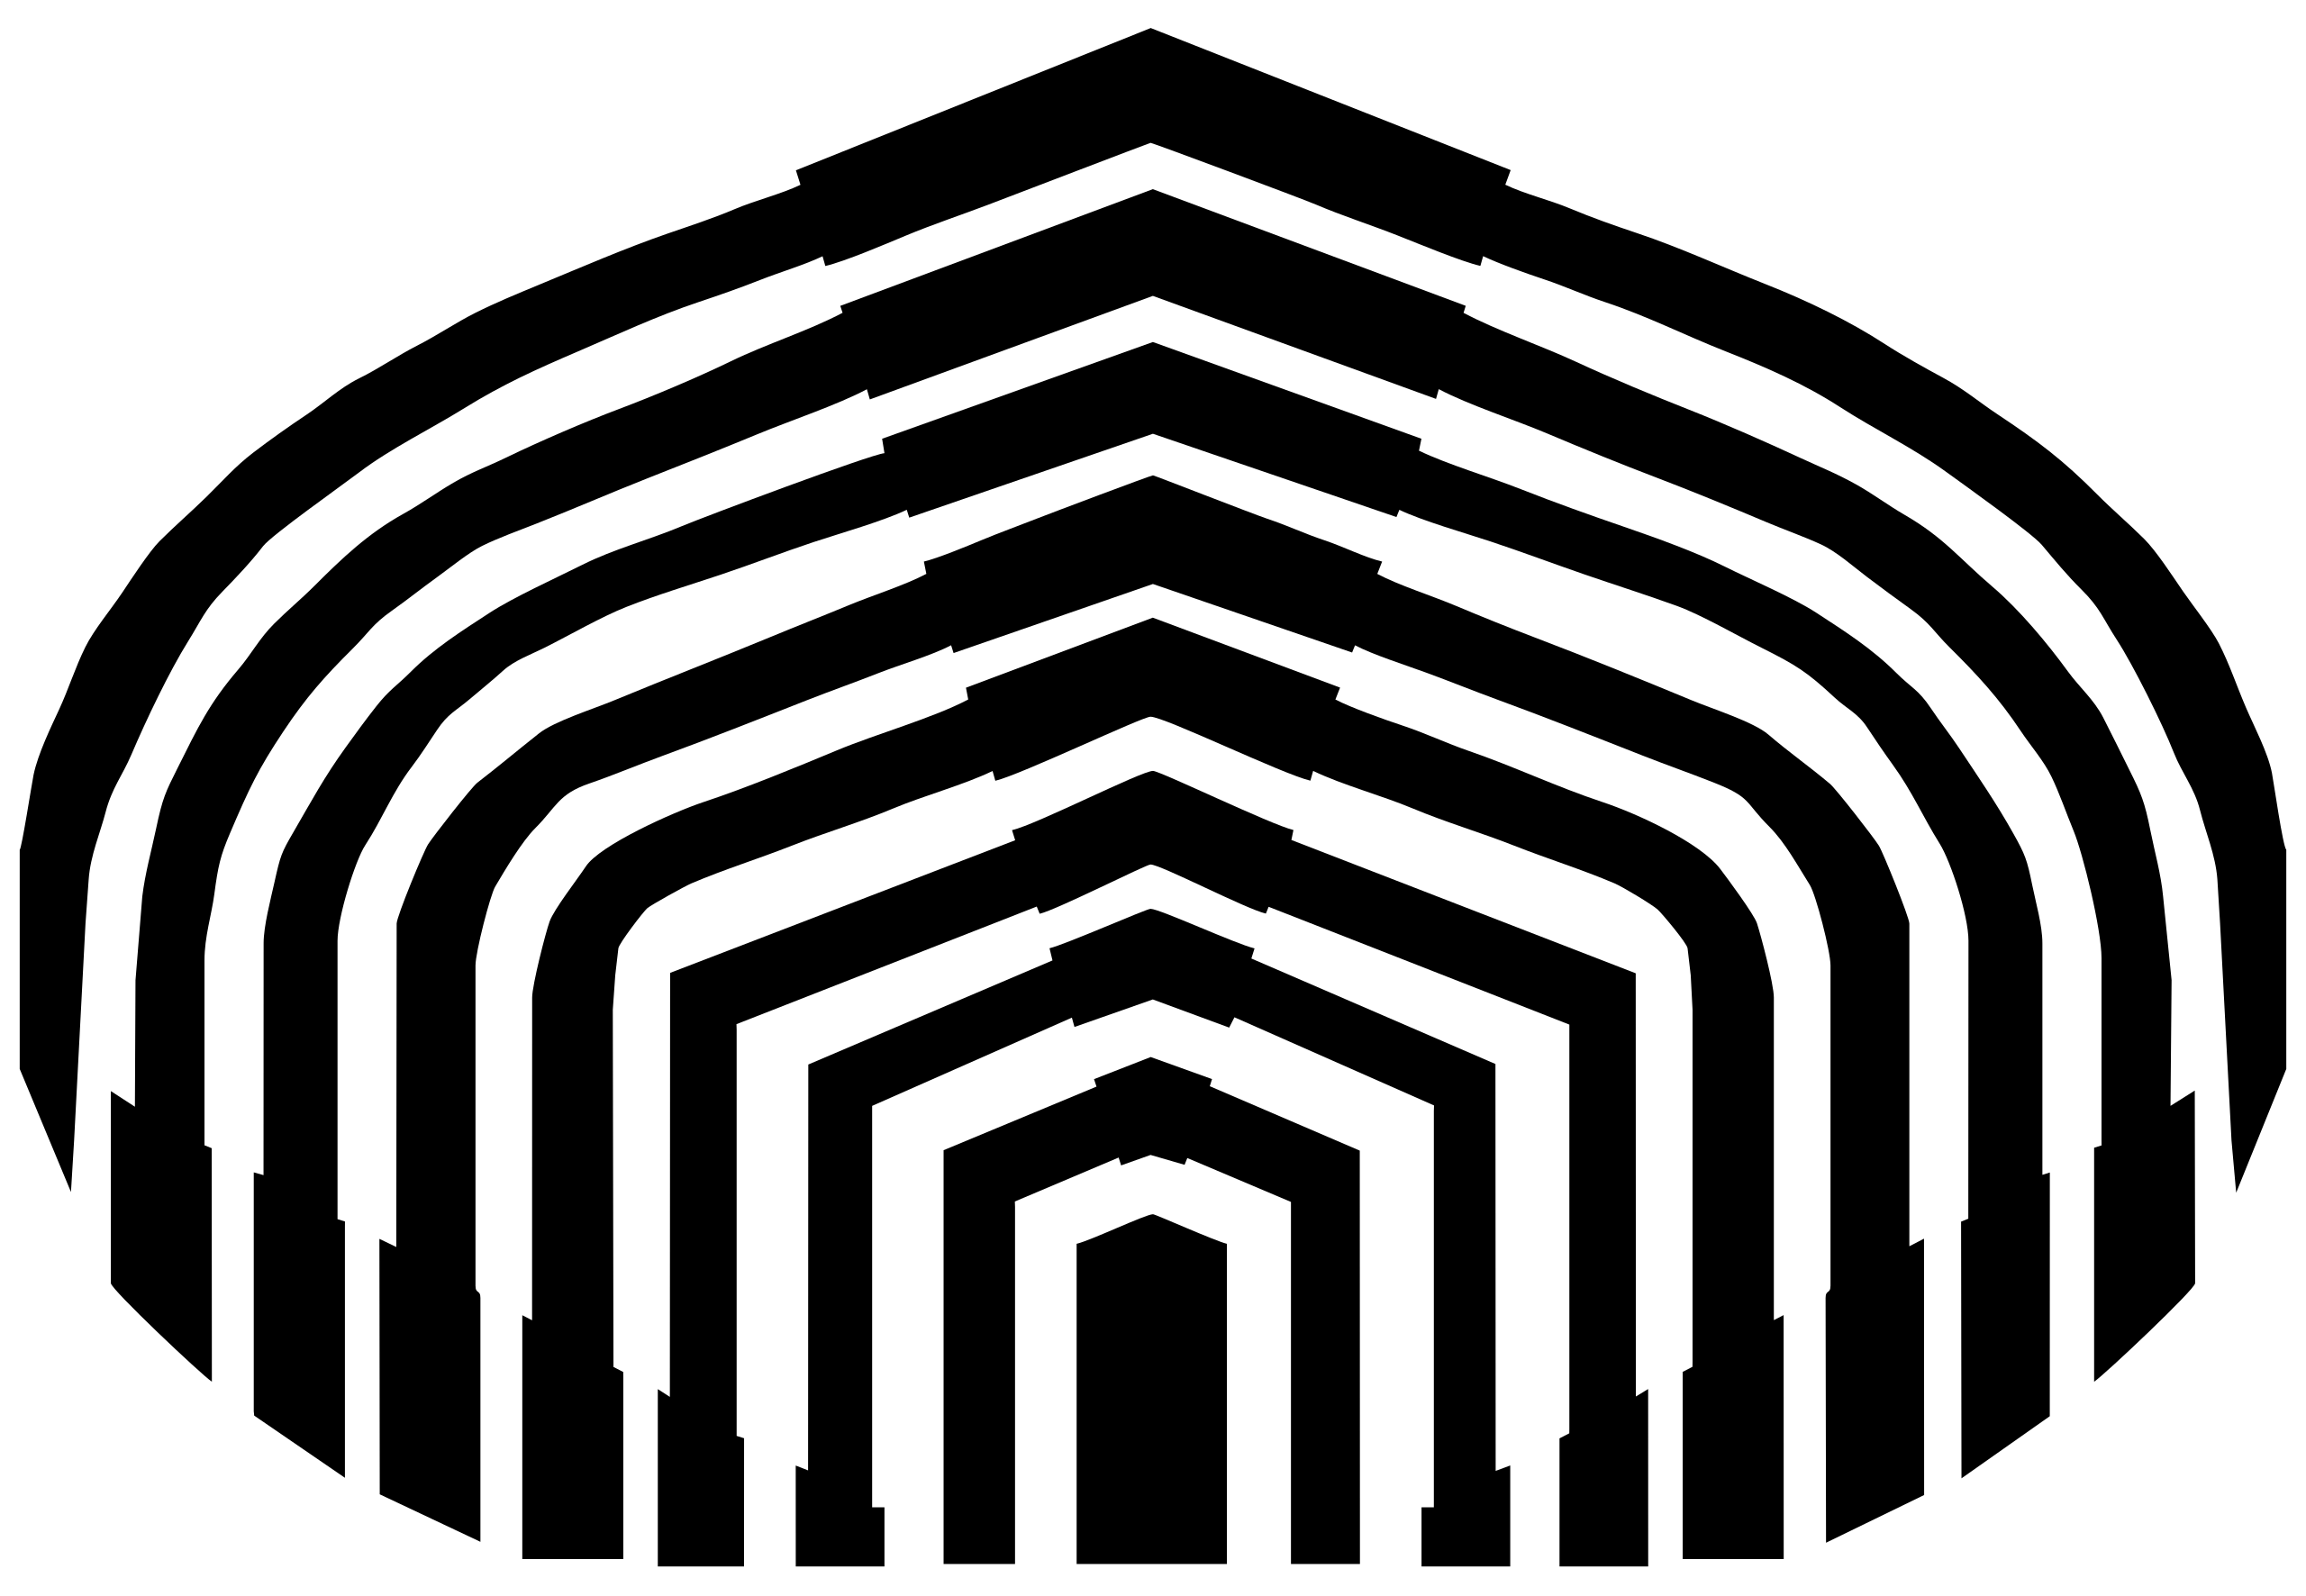
\includegraphics[width=3.1cm,height=2cm]{logo}\\
		UNIVERSIDAD SIMÓN BOLÍVAR\\
		DEPARTAMENTO DE ELECTRÓNICA Y CIRCUITOS\\
		EC1281 - LABORATORIO DE MEDICIONES ELÉCTRICAS\\
		SECCIÓN 1 - GRUPO 1\\
		
		\vspace{7cm}
		\textbf{\Large INFORME - PRÁCTICA \#5}\\
		PRESENTACIÓN X-Y MEDICIONES CON EL OSCILOSCOPIO SOBRE CIRCUITOS RC Y RL\\
	\end{center}
	
	\begin{flushleft}
		\vspace{8cm}
		\hfill Integrantes:\\
		\hfill {\large Luis Becerra - 1910557}\\
		\hfill {\large Lorena Rojas - 1910469}\\
	\end{flushleft}
	
	\newpage
	
	\pagenumbering{Roman}
	\setcounter{page}{2}
	
	\begin{center}
		\textbf{\large RESUMEN}\\
	\end{center}
	
	En esta práctica, se exploró el funcionamiento y las técnicas de medición del osciloscopio. Los objetivos incluyeron el análisis de las características corriente-voltaje de elementos lineales y no lineales, así como la medición de frecuencias y desfasajes utilizando la presentación X-Y. Se llevaron a cabo diversos experimentos, montando circuitos y realizando mediciones con el osciloscopio. Se determinaron las características corriente-voltaje de una resistencia desconocida y un diodo zener, tanto en el dominio del tiempo como en la presentación XY. Además, se realizaron mediciones de desfasajes en circuitos con capacitores e inductores. Las figuras de Lissajous se utilizaron para medir la frecuencia de la línea. Se registraron las mediciones y se tomaron fotografías de las formas de onda y las gráficas obtenidas. En conclusión, la práctica permitió profundizar en el conocimiento del osciloscopio y aplicar técnicas de medición en diversos circuitos.
	
	\newpage
	
	\begin{center}
		\textbf{\large ÍNDICE}\\
	\end{center}
	
	\noindent \textbf{RESUMEN} \hfill \textbf{II}\\
	\noindent \textbf{ÍNDICE} \hfill \textbf{III}\\
	\noindent \textbf{MARCO TEÓRICO} \hfill \textbf{1}\\
	\noindent \textbf{METEDOLOGÍA} \hfill \textbf{4}\\
	\noindent \textbf{RESULTADOS} \hfill \textbf{7}\\
	\noindent \textbf{ANÁLISIS DE RESULTADOS} \hfill \textbf{28}\\
	\noindent \textbf{CONCLUSIONES} \hfill \textbf{29}\\
	\noindent \textbf{BIBLIOGRAFÍA} \hfill \textbf{30}\\
	\noindent \textbf{ANEXOS} \hfill \textbf{31}\\
	
	\newpage
	
	\pagenumbering{arabic}
	
	\begin{center}
		\textbf{\large MARCO TEÓRICO}\\
	\end{center}
	
	\textbf{1. Modalidad XY del osciloscopio}\\
	
	El osciloscopio es un instrumento ampliamente utilizado en el ámbito de la electrónica y las telecomunicaciones para visualizar y medir señales eléctricas. En su modalidad XY (eje X e Y), el osciloscopio permite representar gráficamente la relación entre dos señales en un plano cartesiano, lo cual resulta especialmente útil para analizar las características corriente-voltaje de elementos lineales y no lineales, así como para medir frecuencias y desfasajes utilizando las Figuras de Lissajous.\\
	
	En la modalidad XY, el osciloscopio se utiliza en combinación con un generador de funciones que suministra una señal de voltaje de referencia y un circuito bajo prueba que genera una señal de corriente o voltaje. Estas señales se conectan a los canales X e Y del osciloscopio, respectivamente, y se representan en el plano XY, donde el eje X representa una señal y el eje Y representa la otra señal.\\
	
	\textbf{2. Características corriente-voltaje de elementos lineales}
	
	\begin{itemize}
		\item \textbf{Definición de características corriente-voltaje}
		
		Las características corriente-voltaje, también conocidas como curvas I-V o curvas de transferencia, describen la relación entre la corriente eléctrica que fluye a través de un componente o circuito y la tensión aplicada a dicho componente. Estas características son representativas del comportamiento eléctrico de los elementos y proporcionan información crucial sobre su funcionamiento.
		
		\item \textbf{Medición de la característica corriente-voltaje en elementos lineales}
		
		La medición de la característica corriente-voltaje en elementos lineales se realiza mediante la configuración de un circuito de medición adecuado. El objetivo es aplicar diferentes niveles de tensión al elemento lineal y medir la corriente resultante para obtener los puntos necesarios para trazar la curva I-V.
	\end{itemize}
	
	\textbf{3. Características corriente-voltaje de elementos no lineales}
	
	\begin{itemize}
		\item \textbf{Comportamiento no lineal de los elementos}
		
		A diferencia de los elementos lineales, los elementos no lineales exhiben un comportamiento no proporcional entre la corriente y la tensión aplicada. En otras palabras, la relación entre la corriente y la tensión no sigue una ley lineal, sino que puede ser no lineal y presentar efectos no despreciables, como la distorsión armónica, la rectificación, la conmutación o la generación de armónicos.
		
		El comportamiento no lineal puede ser causado por diversas razones, como la dependencia de la temperatura, la presencia de elementos activos (como transistores o diodos) o la interacción con campos eléctricos o magnéticos. Estos elementos no lineales requieren un análisis específico y una comprensión detallada de sus características corriente-voltaje.
		
		\item \textbf{Medición de la característica corriente-voltaje en elementos no lineales}
		
		La medición de la característica corriente-voltaje en elementos no lineales también implica la configuración de un circuito de medición adecuado. Sin embargo, debido al comportamiento no lineal de estos elementos, se requieren enfoques diferentes para obtener una representación precisa de su curva I-V.
	\end{itemize}
	
	\textbf{4. Medición de frecuencias mediante Figuras de Lissajous}
	
	\begin{itemize}
		\item \textbf{Utilización del osciloscopio en modalidad XY para medir frecuencias}
		
		El osciloscopio en modalidad XY es una herramienta útil para medir y visualizar las frecuencias de señales eléctricas. Esta modalidad permite representar las señales en un plano cartesiano, donde el eje X representa una señal de referencia y el eje Y representa la señal a medir. La relación entre estas dos señales da lugar a las Figuras de Lissajous.
		
		\item \textbf{Interpretación de las Figuras de Lissajous y cálculo de frecuencias}
		
		Las Figuras de Lissajous proporcionan información visual sobre la relación de frecuencias entre la señal de referencia y la señal a medir. Dependiendo de la forma de la figura resultante, es posible determinar si las frecuencias son iguales, proporcionales o están en relación armónica.
		
		Para calcular las frecuencias utilizando las Figuras de Lissajous, se utiliza la fórmula: $$f_{2} = (n_{2}/n_{1}) * f_{1}$$
		
		Donde $f_{2}$ es la frecuencia de la señal a medir, $f_{1}$ es la frecuencia de la señal de referencia, $n_{1}$ es el número de cruces de la señal de referencia en el eje X y $n_{2}$ es el número de cruces de la señal a medir en el eje Y.
		
		Este cálculo permite determinar la frecuencia de la señal a medir en función de la frecuencia de referencia y la relación geométrica de las Figuras de Lissajous.
		
	\end{itemize}
	
	
	\textbf{5. Medición de desfasajes mediante Figuras de Lissajous}
	
	\begin{itemize}
		\item \textbf{Utilización del osciloscopio en modalidad XY para medir desfasajes}
		
		El osciloscopio en modalidad XY también puede utilizarse para medir desfasajes entre dos señales eléctricas. Las Figuras de Lissajous generadas en el plano cartesiano proporcionan información visual sobre el desfase relativo entre las señales.
		
		\item \textbf{Interpretación de las Figuras de Lissajous y cálculo de desfasajes}
		
		Las Figuras de Lissajous proporcionan información visual sobre el desfasaje entre las señales de referencia y a medir. Dependiendo de la forma y la inclinación de la figura resultante, es posible determinar el desfasaje y su naturaleza (positivo o negativo).
		
		La medición de desfasajes mediante Figuras de Lissajous es una técnica valiosa en el análisis de circuitos y sistemas. Proporciona una representación visual intuitiva de los desfasajes y permite obtener mediciones precisas y confiables de las diferencias de fase entre las señales en estudio.
	\end{itemize}
	
	\textbf{6. Medición de constantes de tiempo mediante cursores del osciloscopio}
	
	\begin{itemize}
		\item \textbf{Definición de constantes de tiempo en circuitos RC y RL}
		
		Las constantes de tiempo son parámetros importantes en circuitos RC (resistencia-capacitancia) y RL (resistencia-inductancia). Representan el tiempo necesario para que ciertas magnitudes eléctricas alcancen un determinado valor en respuesta a un cambio en el circuito.
		En un circuito RC, la constante de tiempo ($\tau$) se define como el producto de la resistencia (R) y la capacitancia (C), y se expresa en segundos (s). Indica el tiempo requerido para que el voltaje o la corriente en el circuito alcancen aproximadamente el 63.2\% de su valor final después de un cambio en la señal de entrada.
		
		En un circuito RL, la constante de tiempo ($\tau$) se define como el cociente entre la inductancia (L) y la resistencia (R), y también se mide en segundos (s). Representa el tiempo necesario para que la corriente en el circuito alcance aproximadamente el 63.2\% de su valor final después de un cambio en la señal de entrada.
		
		\item \textbf{Cálculo de las constantes de tiempo}
		
		Se debe medir el tiempo requerido para que el voltaje alcance el 63.2\% de su valor final.
		
		Luego, utilizando la fórmula correspondiente según el tipo de circuito (RC o RL), se puede calcular la constante de tiempo.
		
		Para un circuito RC, la fórmula es: $$\tau = R * C$$
		
		Para un circuito RL, la fórmula es: $$\tau = L / R$$
		
		Realizando los cálculos apropiados con los valores medidos, se obtendrá la constante de tiempo del circuito.
	\end{itemize}
	
	\newpage
	
	\begin{center}
		\textbf{\large METODOLOGÍA}\\
	\end{center}
	
	En la metodología se llevaron a cabo los siguientes procedimientos y se utilizaron los siguientes circuitos, junto con los valores nominales de los componentes empleados:\\
	
	\textbf{1. Configuración del circuito para medir las características corriente-voltaje de elementos lineales:}
	
	\begin{itemize}
		\item Se utilizó un circuito serie con una fuente de voltaje DC, un resistor y un voltímetro.
		\item Los valores nominales de los componentes fueron: fuente de voltaje DC de 10V, resistor de $1k\Omega$ y voltímetro de rango adecuado.
		\item La fuente de tensión proporciona la tensión de entrada variable, que se aplica al elemento lineal. El voltimetro se coloca en paralelo para medir el voltaje que fluye a través del elemento. Se debe asegurar que el voltimetro tenga una resistencia interna baja para evitar perturbaciones significativas en el circuito y obtener mediciones precisas.
		\item Al variar la tensión de entrada y medir la corriente resultante, se pueden obtener varios puntos en la curva I-V. Estos puntos se pueden graficar para visualizar la relación entre la corriente y la tensión y analizar el comportamiento lineal del elemento. 
	\end{itemize}
	
	\textbf{2. Configuración del circuito para medir las características corriente-voltaje de elementos no lineales:}
	
	\begin{itemize}
		\item Se utilizó un circuito serie con una fuente de voltaje DC, un diodo y un voltímetro.
		\item Los valores nominales de los componentes fueron: fuente de voltaje DC de 10V, diodo de 4,3V y voltímetro de rango adecuado.
		\item La fuente de tensión variable se utiliza para aplicar diferentes niveles de tensión al diodo, mientras que el osciloscopio muestra la forma de onda de la corriente resultante. Esto permite analizar y comprender el comportamiento no lineal del elemento en función de la tensión aplicada. 
	\end{itemize}
	
	\textbf{3. Configuración del circuito para medir frecuencias mediante Figuras de Lissajous:}
	
	\begin{itemize}
		\item Se utilizó un circuito serie con una fuente de señal AC, un resistor y un osciloscopio en modalidad XY.
		\item Los valores nominales de los componentes fueron: fuente de señal AC con frecuencia variable, resistor de $1k\Omega$ y osciloscopio con capacidad de operar en modalidad XY.
		\item Para medir frecuencias utilizando el osciloscopio en modalidad XY implica conectar la señal de referencia al canal X del osciloscopio y la señal a medir al canal Y. Es importante asegurarse de que ambas señales estén sincronizadas correctamente.
		\item Además, es necesario ajustar los controles de base de tiempo y de amplitud para asegurarse de que las señales se visualicen correctamente en el plano cartesiano.	
		\item Una vez configurado el circuito, se puede proceder a medir las frecuencias utilizando las Figuras de Lissajous. Para ello, se varía la frecuencia de la señal a medir y se observa la forma resultante en el osciloscopio.
		\item Se deben registrar los valores correspondientes de la frecuencia de la señal de referencia y la frecuencia de la señal a medir para cada configuración. Esto permitirá calcular la relación entre las frecuencias y obtener información precisa sobre la señal en cuestión.
	\end{itemize}
	
	\textbf{4. Configuración del circuito para medir desfasajes mediante Figuras de Lissajous:}
	
	\begin{itemize}
		\item Se utilizó un circuito serie con dos fuentes de señal AC, dos resistores y un osciloscopio en modalidad XY.
		\item Los valores nominales de los componentes fueron: dos fuentes de señal AC con frecuencia variable, dos resistores de $1k\Omega$ cada uno y osciloscopio con capacidad de operar en modalidad XY.
		\item Se deben conectar las dos señales cuyo desfase se desea medir a los canales X e Y del osciloscopio. Asegurandose de que ambas señales estén sincronizadas correctamente.
		\item Ajustar los controles de base de tiempo y de amplitud es necesario para obtener una visualización adecuada de las Figuras de Lissajous en el plano cartesiano.
		\item Una vez configurado el circuito, se puede proceder a medir los desfasajes utilizando las Figuras de Lissajous. Para ello, se varía la fase de la señal a medir y se observa la forma resultante en el osciloscopio.
	\end{itemize}
	
	\textbf{5. Configuración del circuito para medir constantes de tiempo mediante cursores del osciloscopio:}
	
	\begin{itemize}
		\item Se utilizó un circuito serie con una fuente de voltaje DC, un resistor y un capacitor o inductor.
		\item Los valores nominales de los componentes fueron: fuente de voltaje DC de 10V, resistor de $1k\Omega$ y capacitor o inductor con valores específicos según el tipo de circuito (RC o RL) y la constante de tiempo a medir.
		\item Es importante tener en cuenta los valores de resistencia, capacitancia o inductancia necesarios para el cálculo de la constante de tiempo deseada.
		\item Una vez configurado el circuito, se pueden utilizar los cursores del osciloscopio para medir las constantes de tiempo.
		\item El procedimiento de medición implica ubicar los cursores en los puntos de inicio y fin de la respuesta temporal del circuito.	
		\item Una vez que se han ubicado los cursores, el osciloscopio proporcionará automáticamente la diferencia de tiempo entre los dos puntos seleccionados y se hace empleo de la formula para calcular la constante de tiempo.	
		
	\end{itemize}
	
	En cada caso, se siguieron los procedimientos estándar para la conexión y ajuste de los circuitos, tomando en cuenta los valores nominales de los componentes mencionados
	
	\newpage
	
	\begin{center}
		\textbf{\large RESULTADOS}\\
	\end{center}
	
	\noindent Los datos obtenidos son:
	
	\begin{center}
		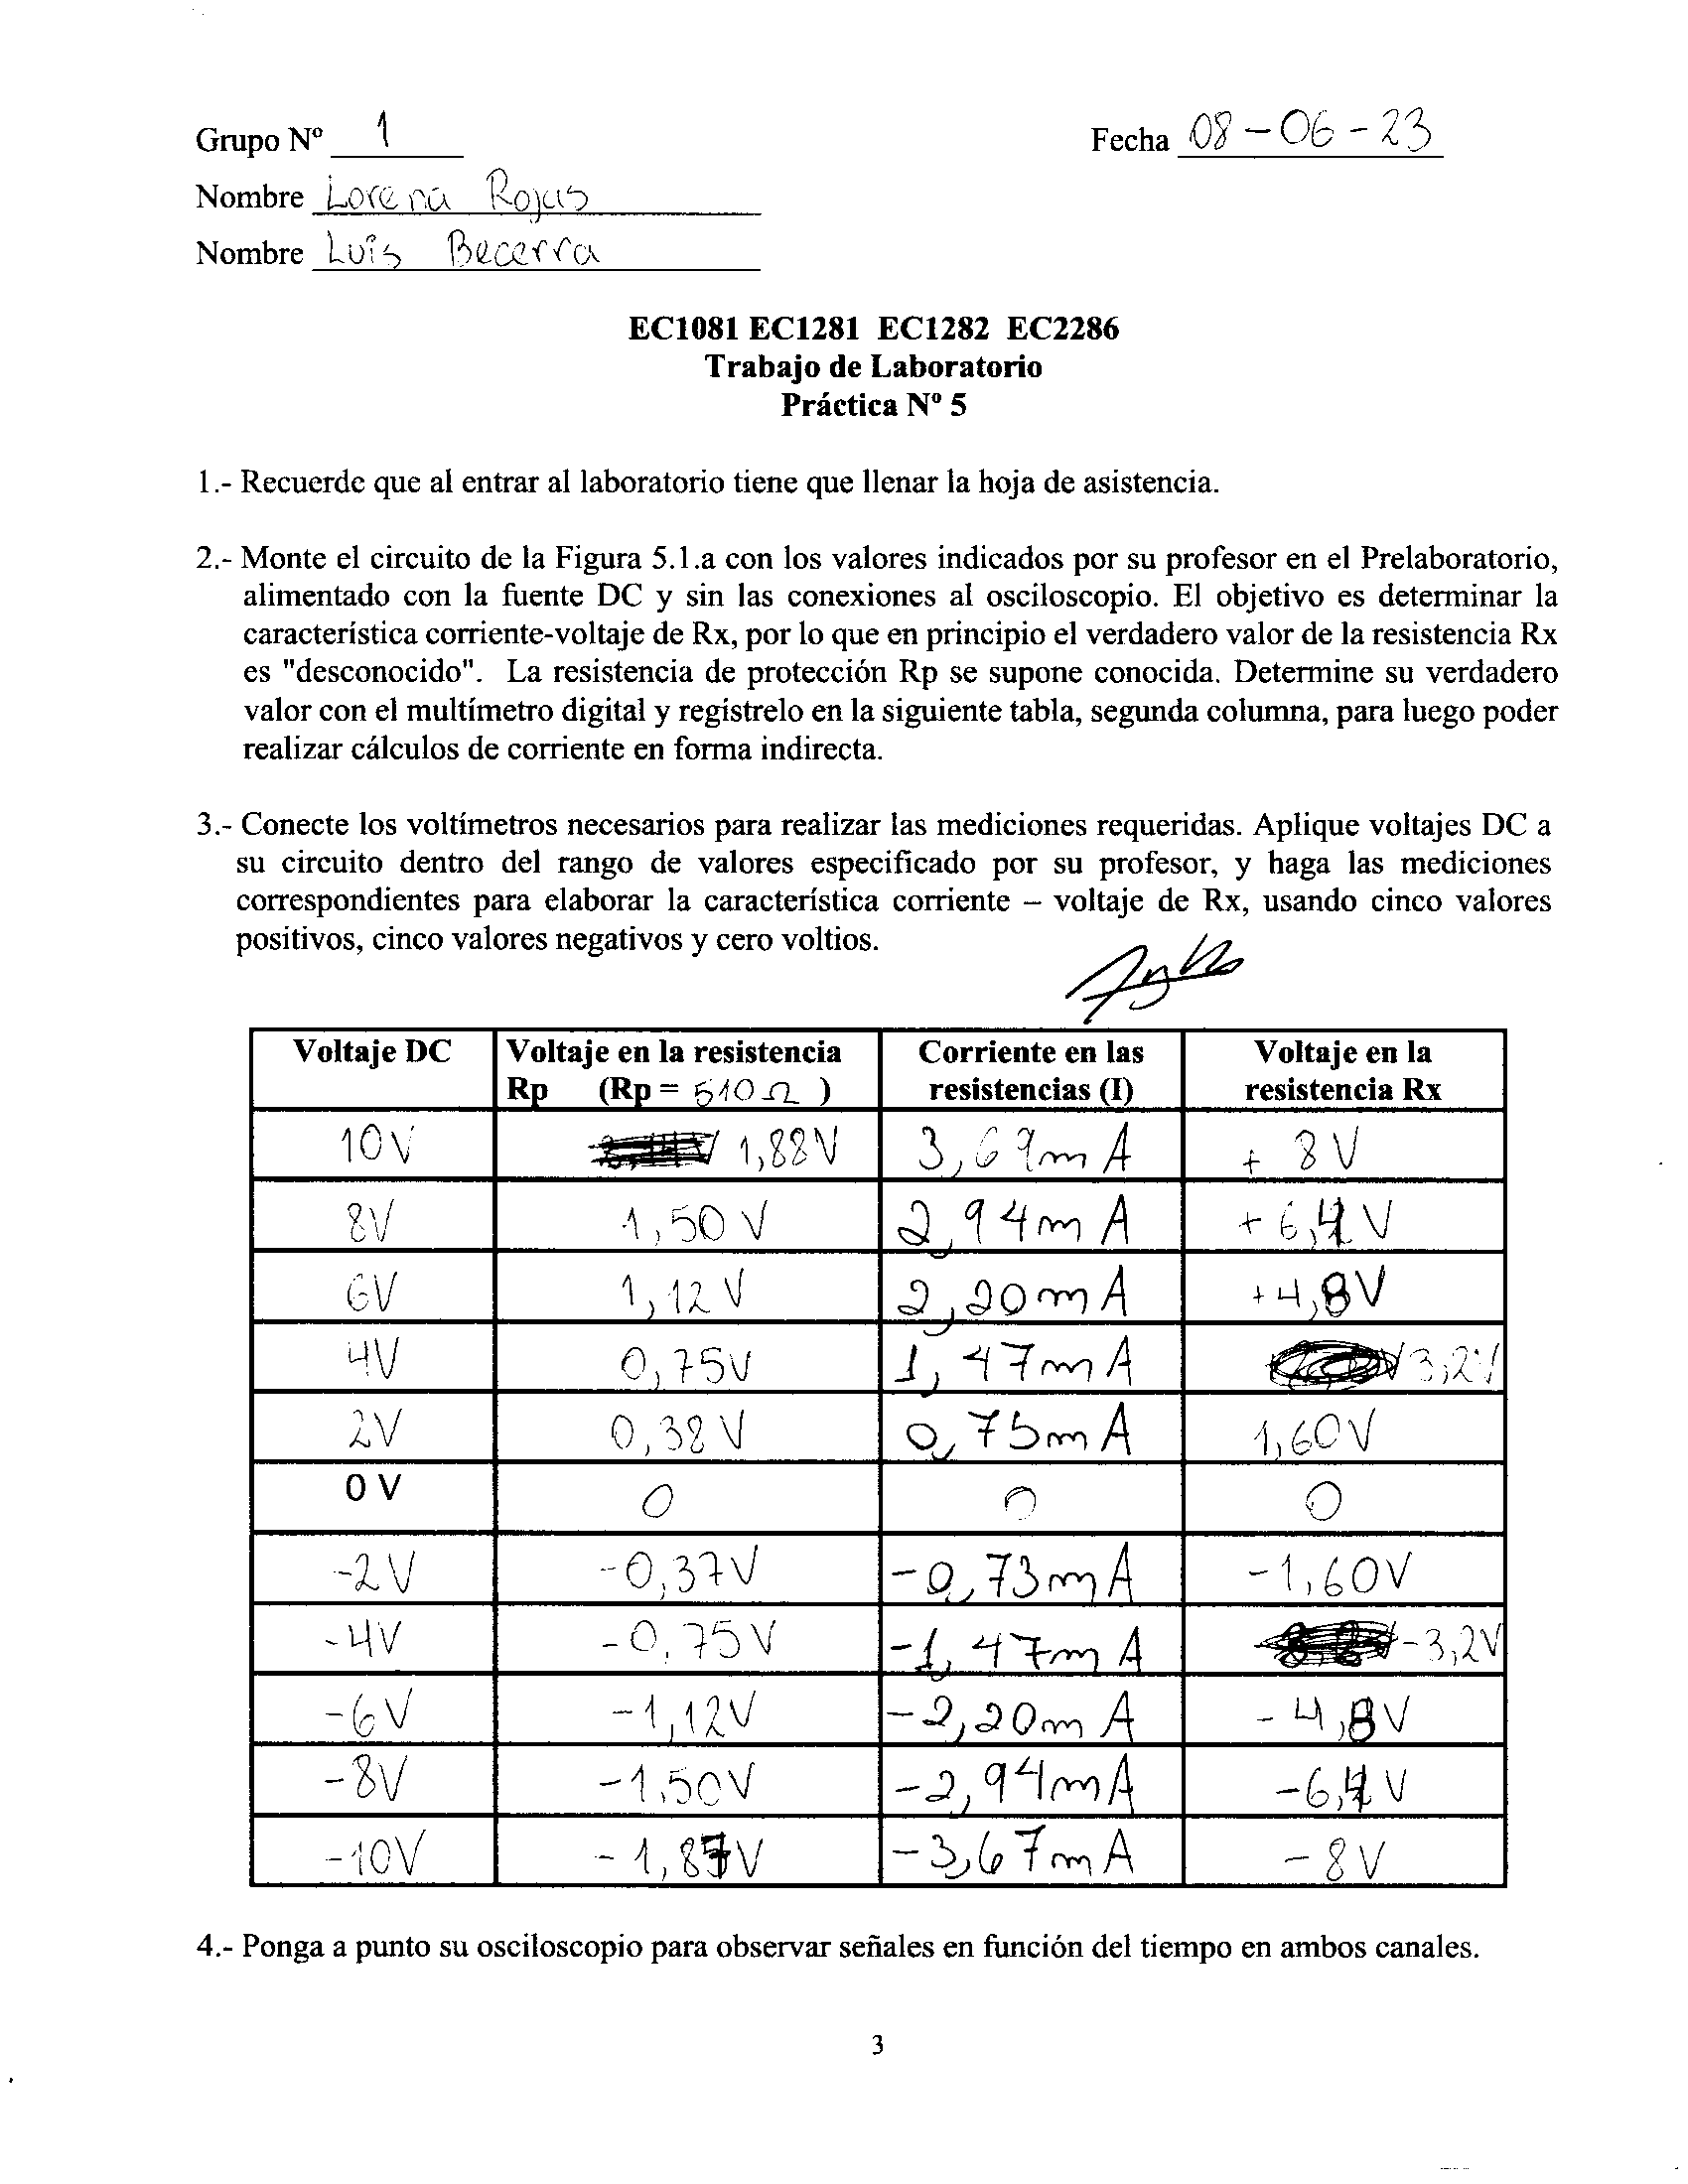
\includegraphics[width=16cm,height=20cm]{Img/anexo_0001}
	\end{center}
	
	\begin{center}
		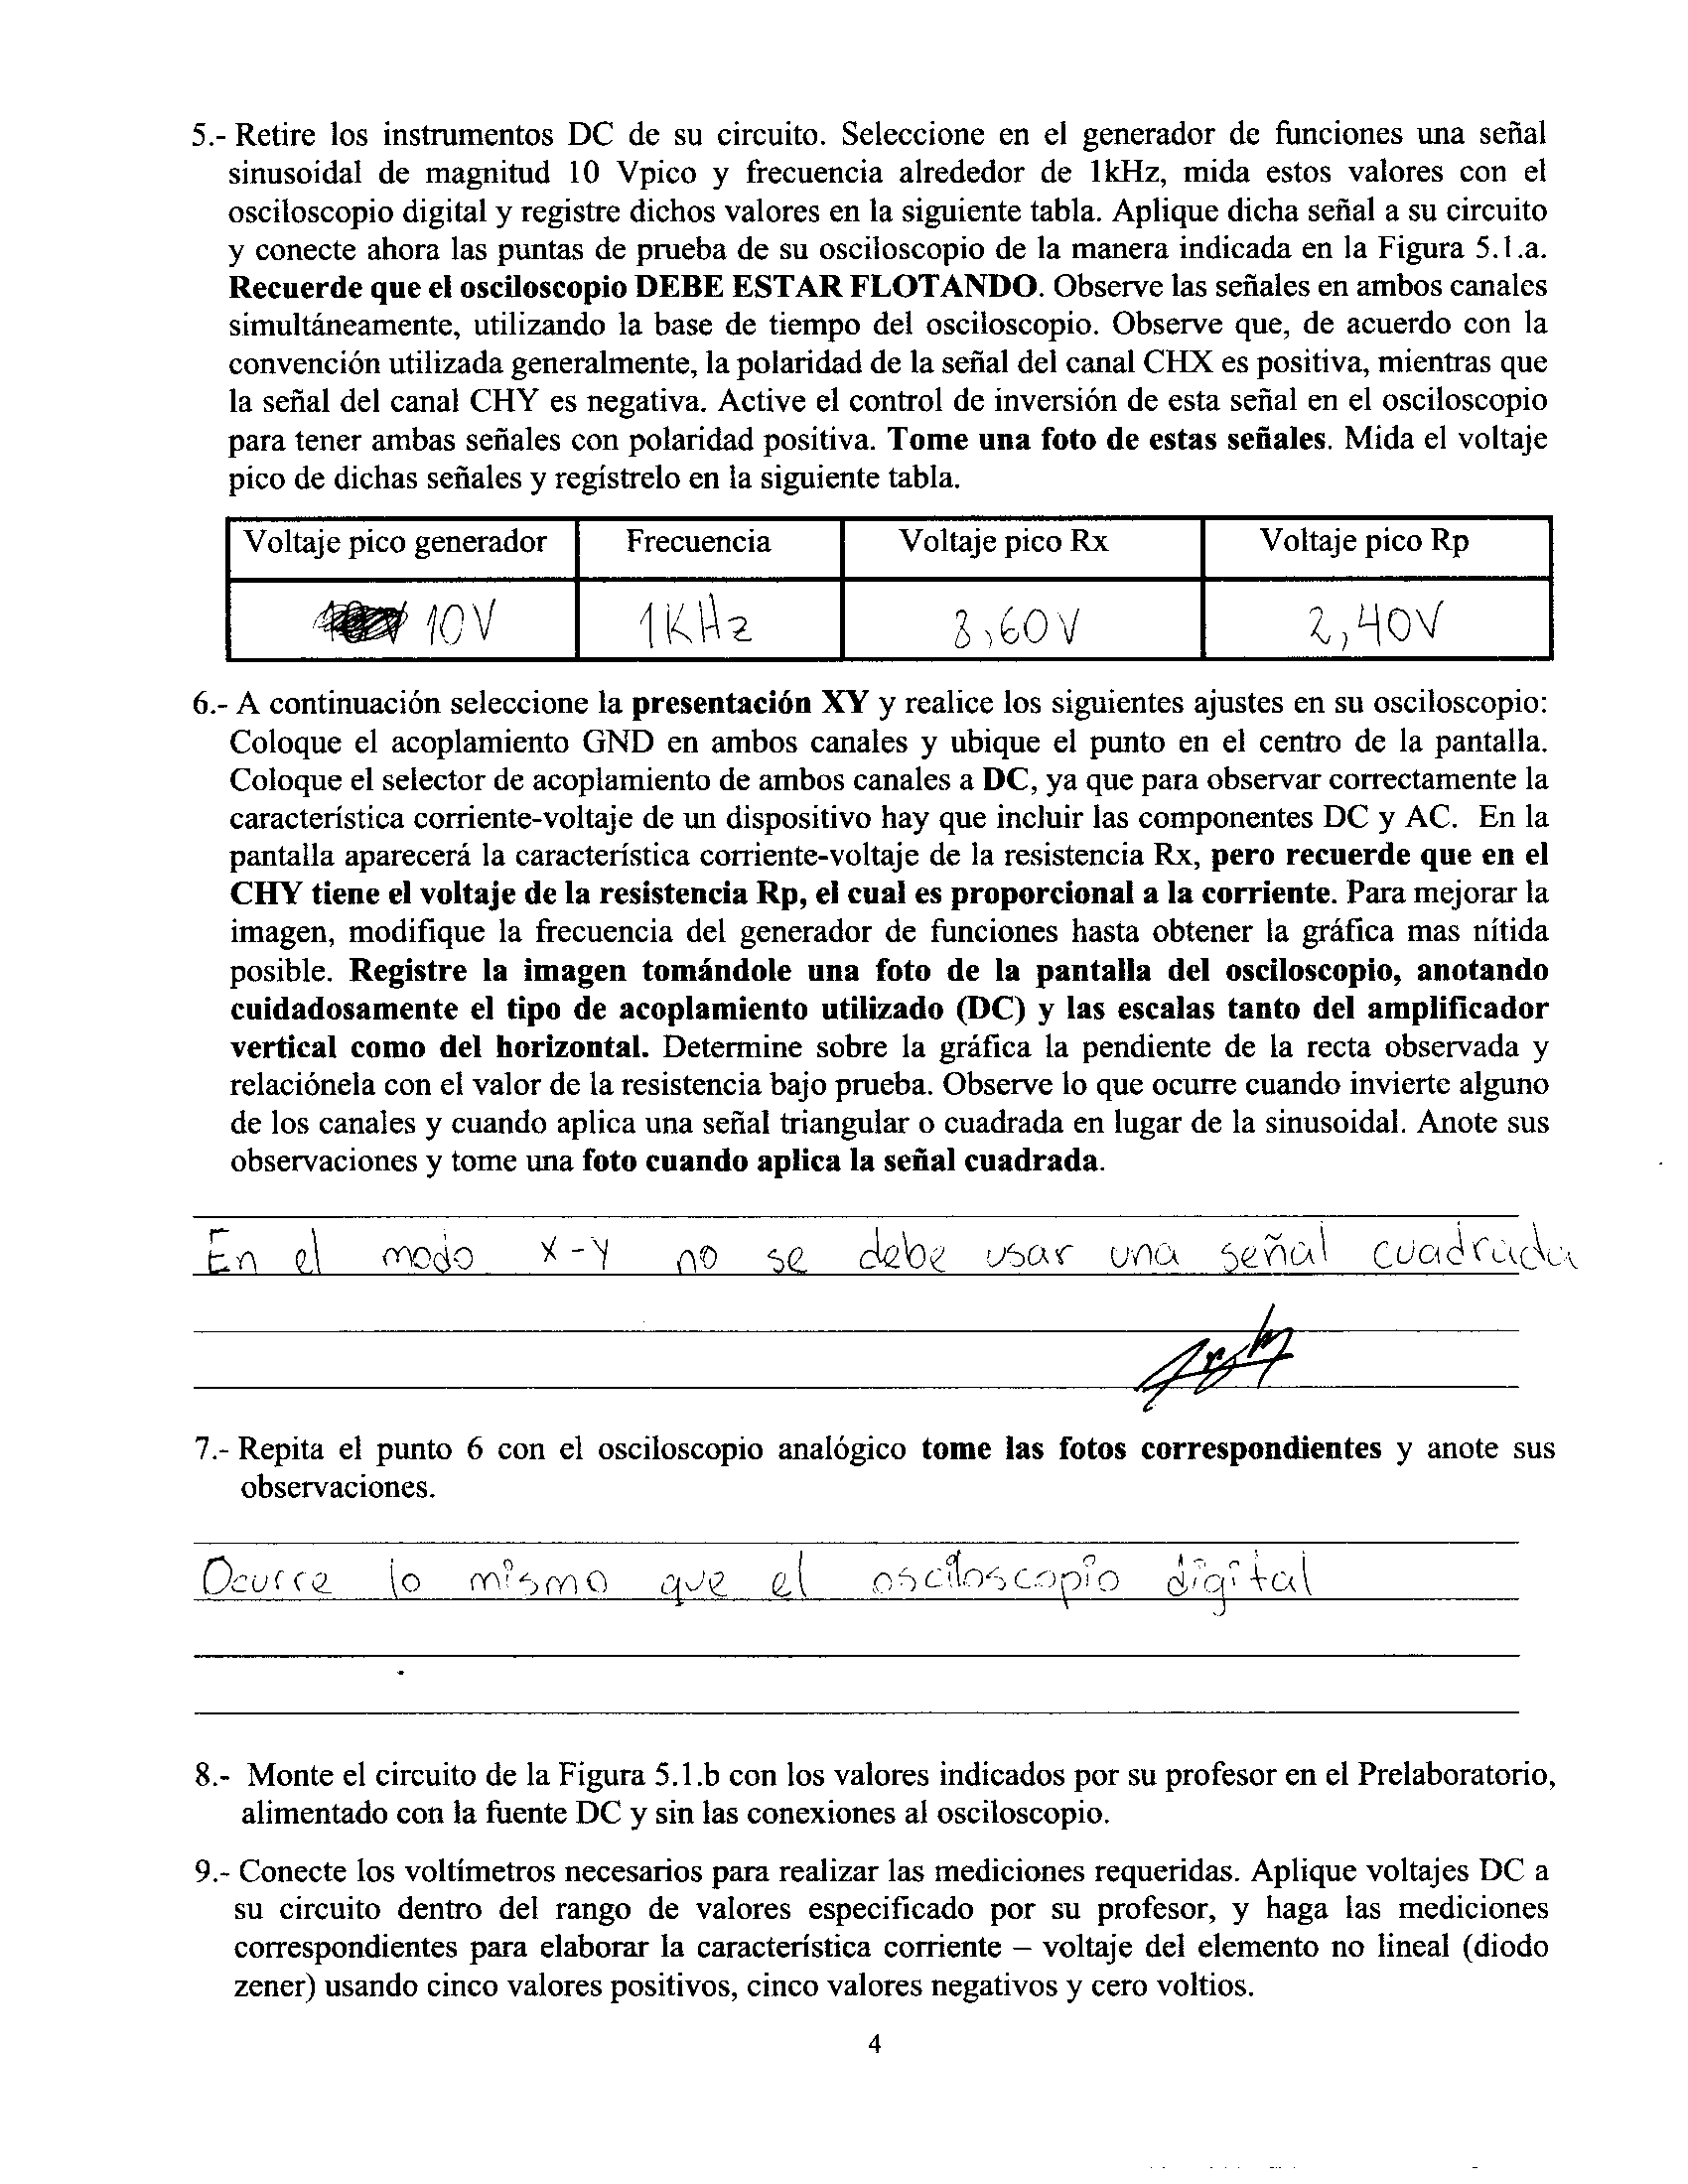
\includegraphics[width=16cm,height=20cm]{Img/anexo_0002}
	\end{center}
	
	\newpage
	
	\noindent Del primer circuito se tomaron las siguientes fotos del osciloscopio: 
	
	\begin{enumerate}
		
		\item Voltaje en cada resistencia modo temporal, osciloscopio digital:
		
		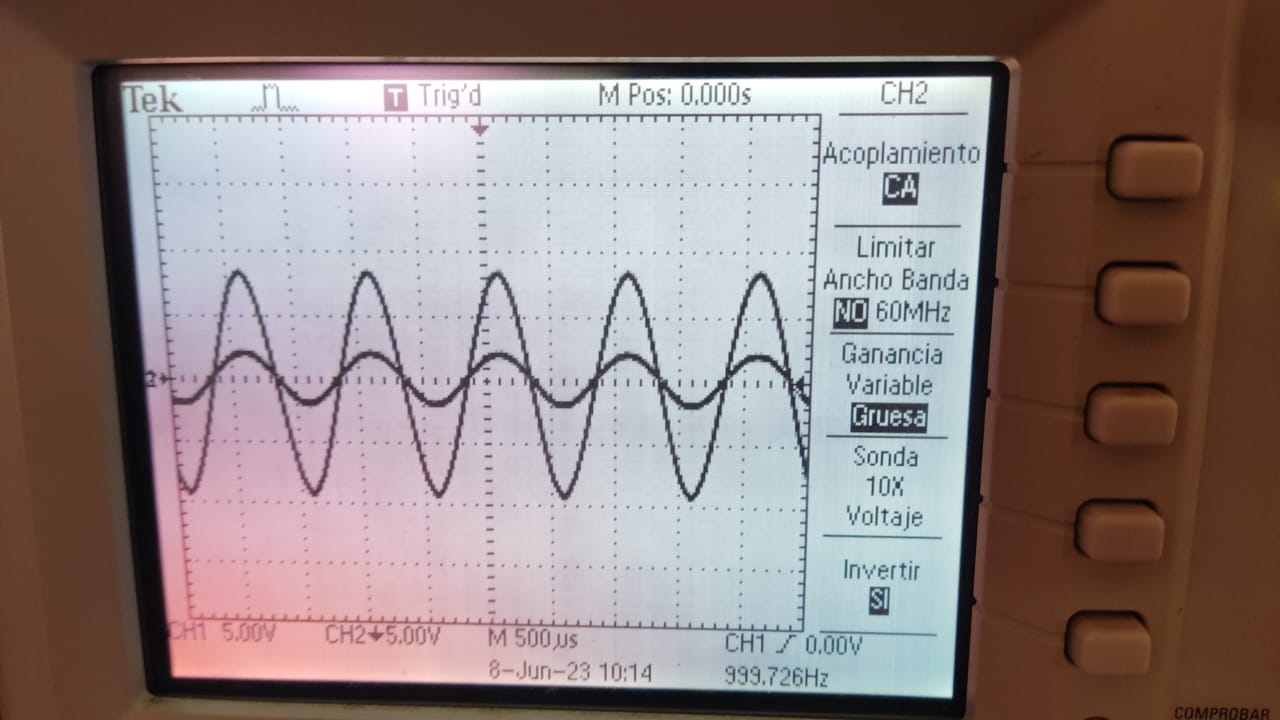
\includegraphics[width=12cm,height=7cm]{Img/lab_5_img_1}
		
		\item Voltaje en cada resistencia modo xy, osciloscopio digital:
		
		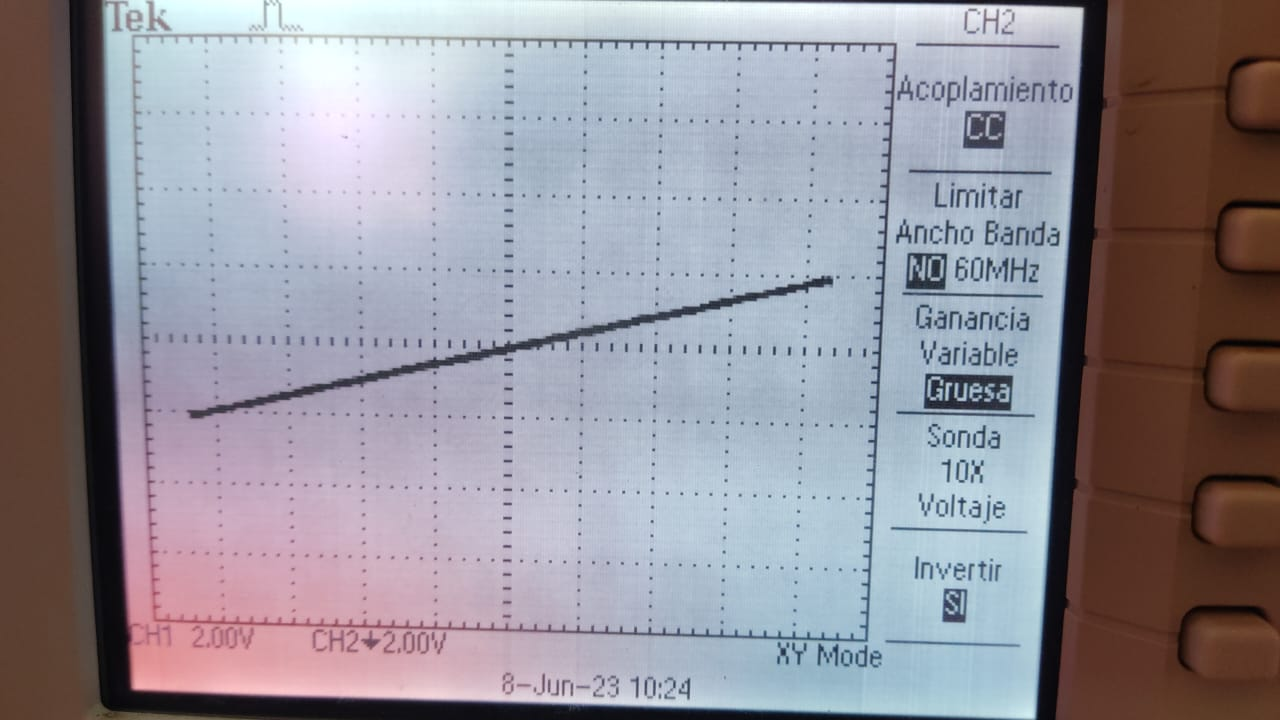
\includegraphics[width=12cm,height=7cm]{Img/lab_5_img_2}
		
		\item Voltaje en cada resistencia modo xy, onda cuadrada, osciloscopio digital:
		
		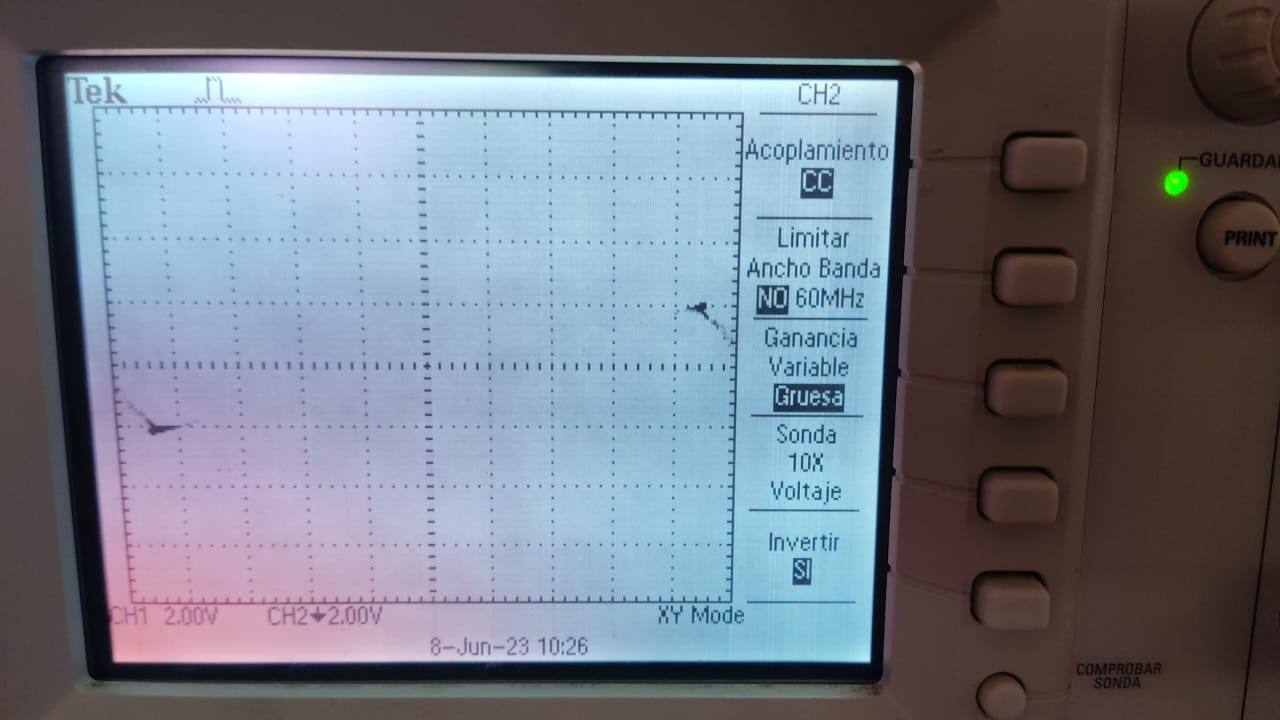
\includegraphics[width=12cm,height=7cm]{Img/lab_5_img_3}
		
		\item Voltaje en cada resistencia modo xy, osciloscopio analógico:
		
		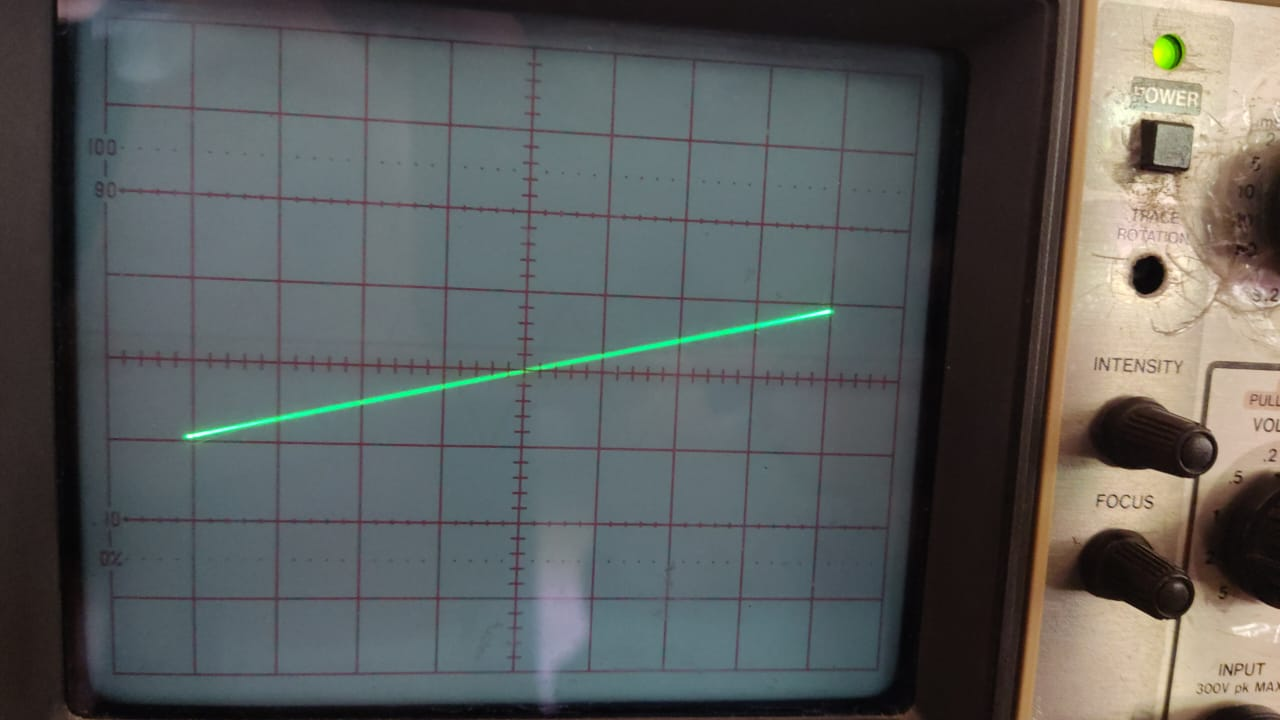
\includegraphics[width=12cm,height=7cm]{Img/lab_5_img_4}
		
		\item Voltaje en cada resistencia modo xy, onda cuadrada, osciloscopio analógico:
		
		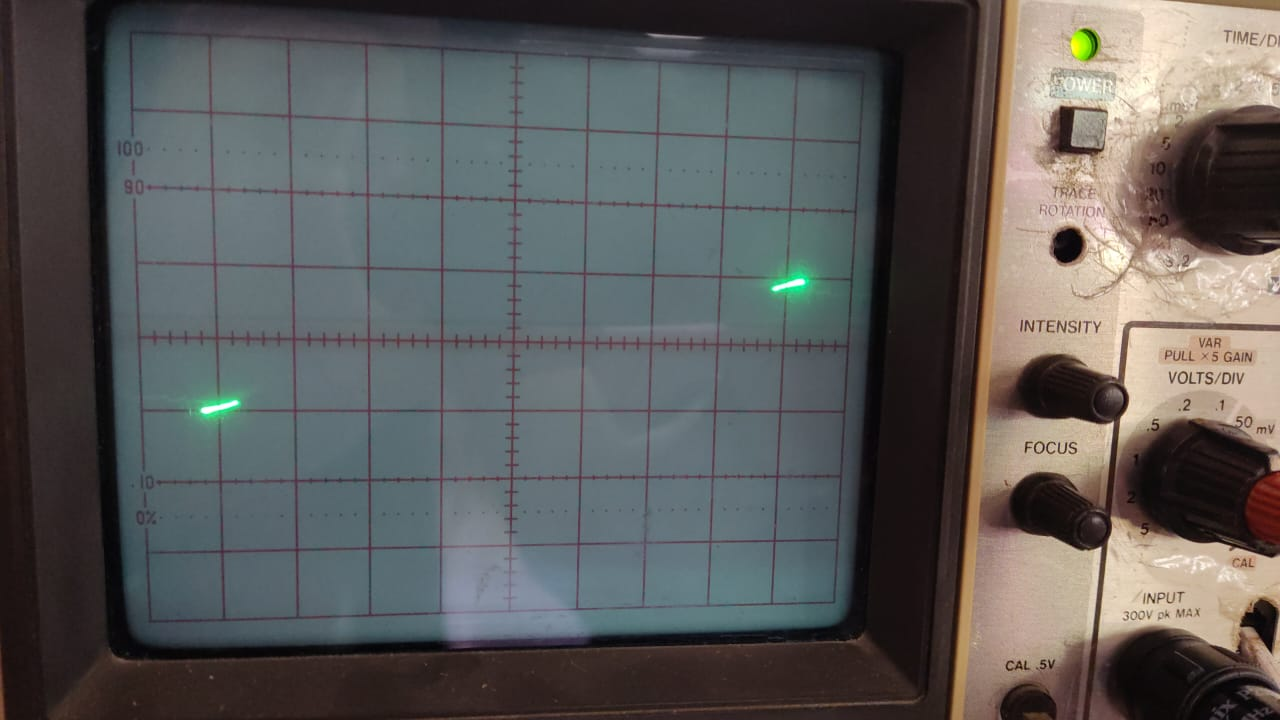
\includegraphics[width=12cm,height=7cm]{Img/lab_5_img_5}
		
	\end{enumerate}
	
	\newpage
	
	\begin{center}
		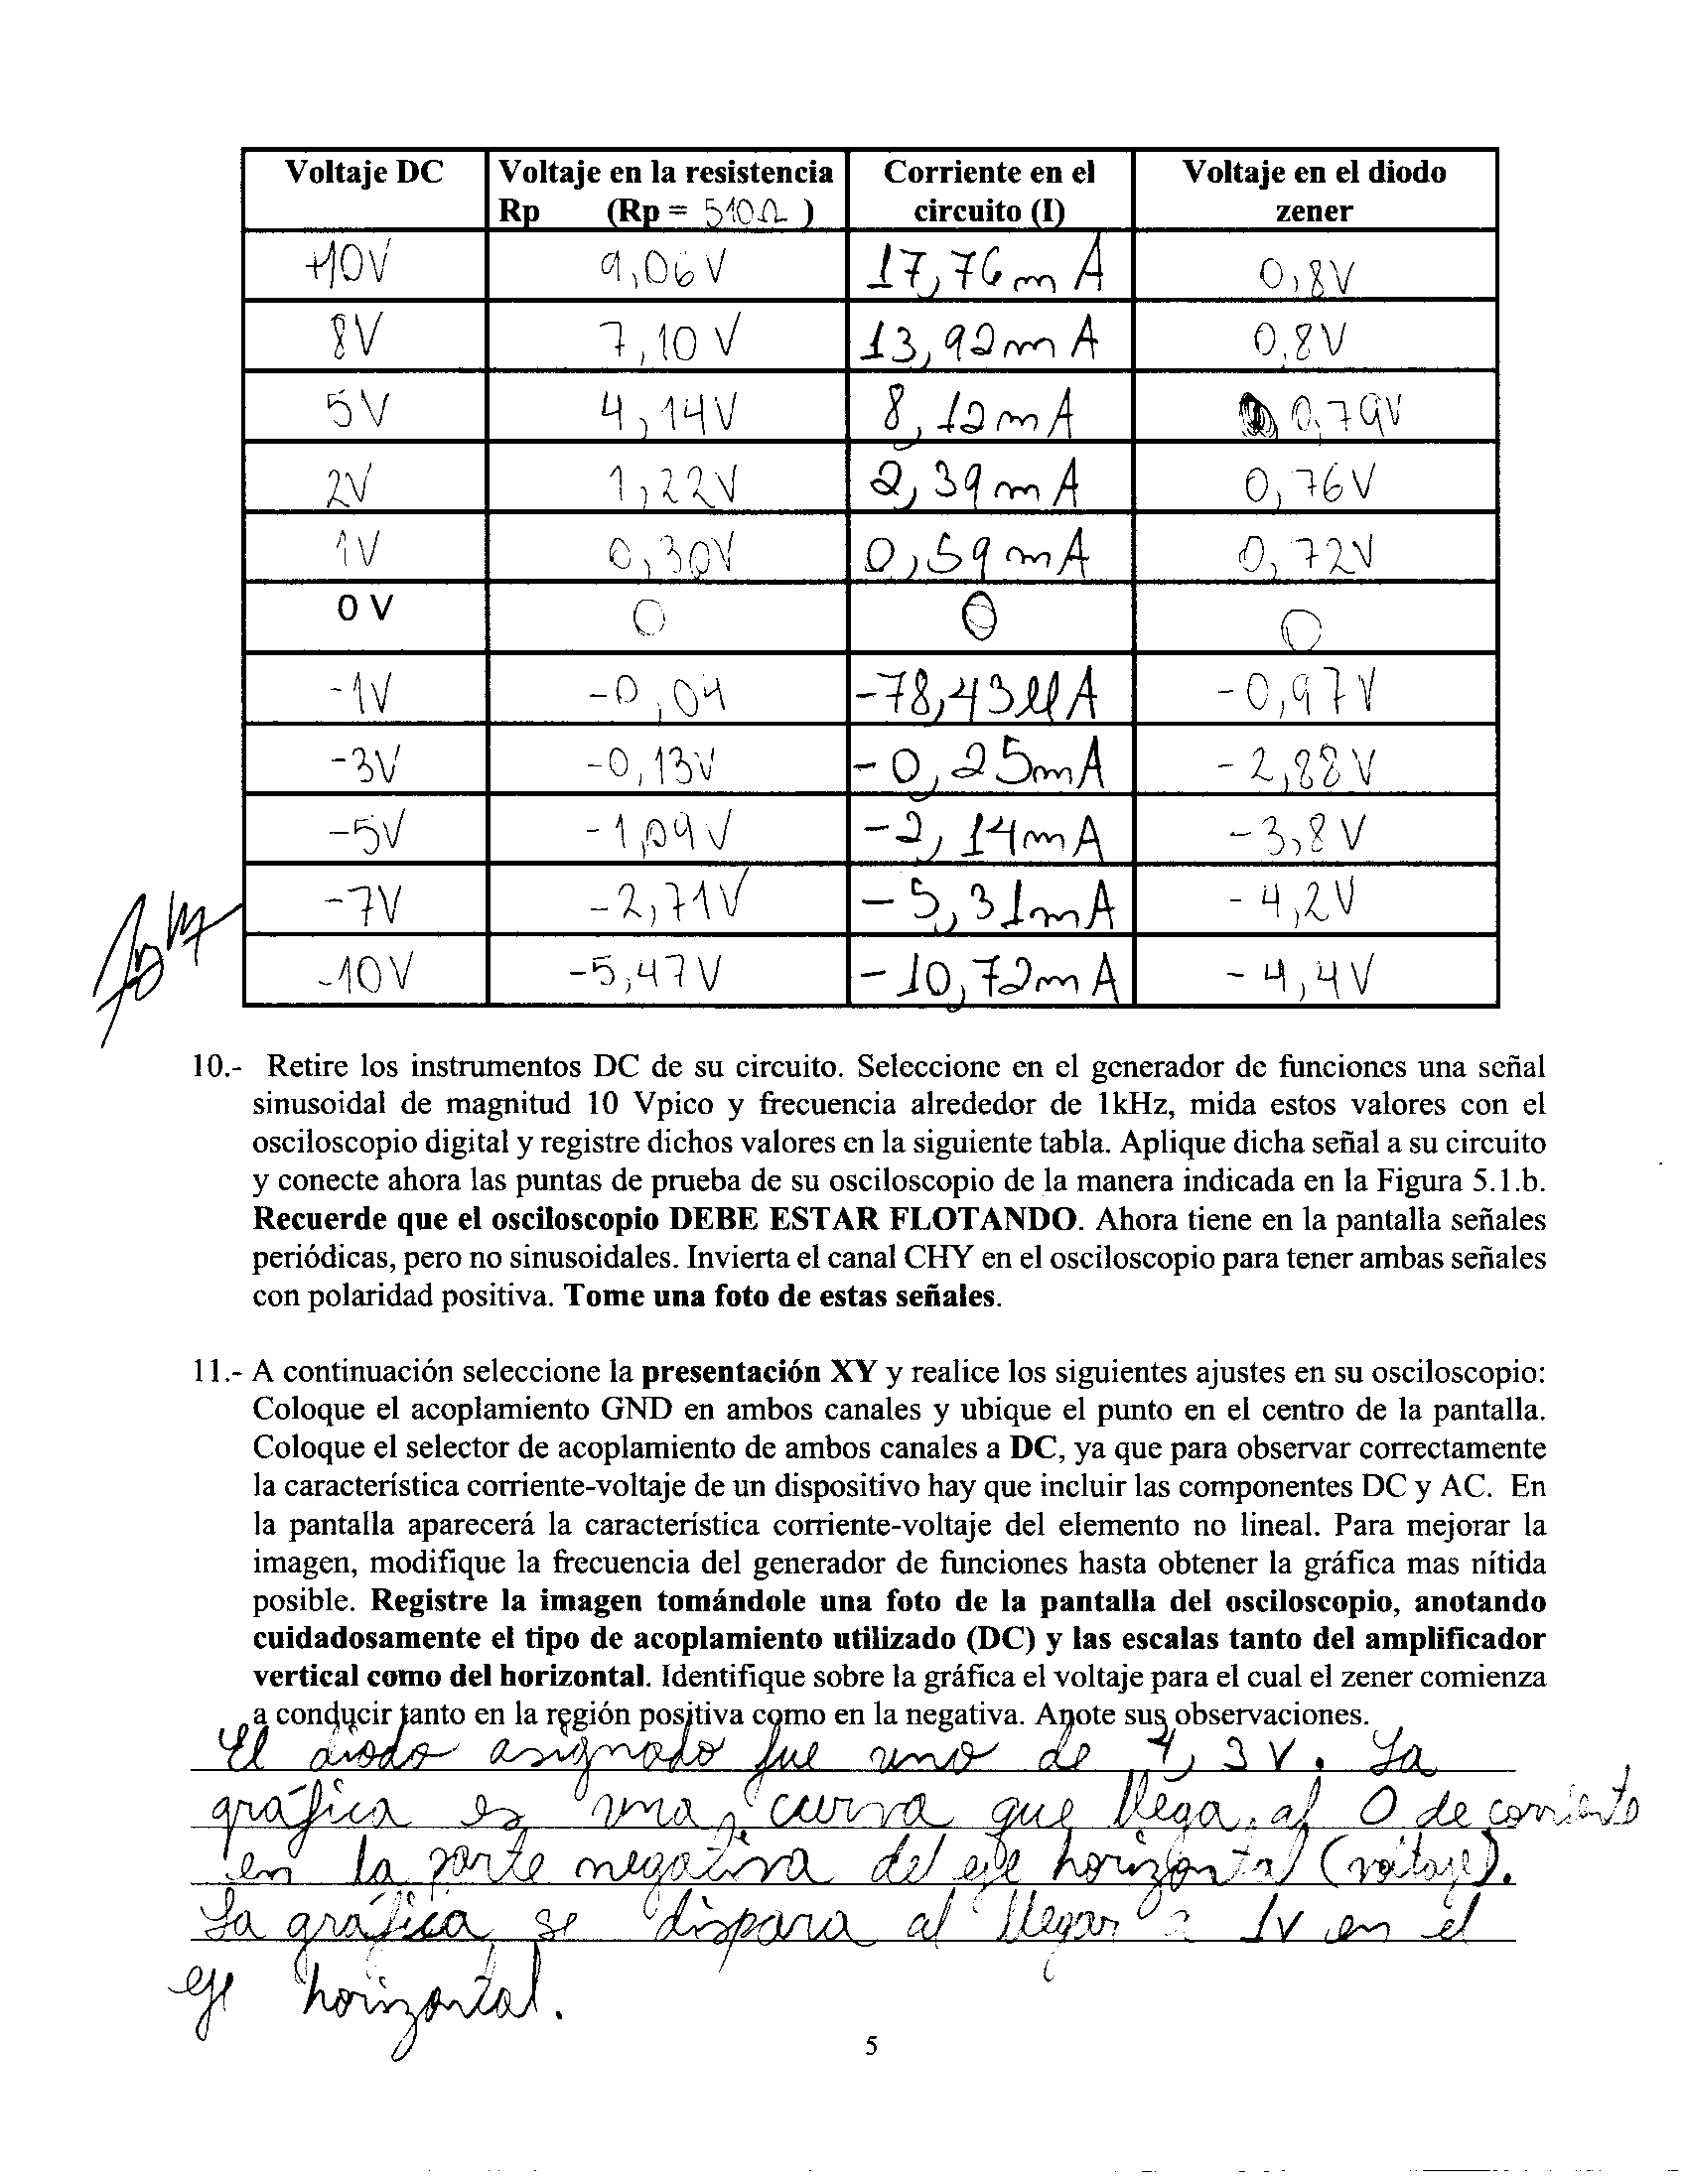
\includegraphics[width=16cm,height=20cm]{Img/anexo_0003}
	\end{center}
	
	\noindent Por otro lado, del circuito con el diodo se obtuvo:
	
	\begin{enumerate}
		\item Voltaje en resistencia y diodo, modo temporal:
		
		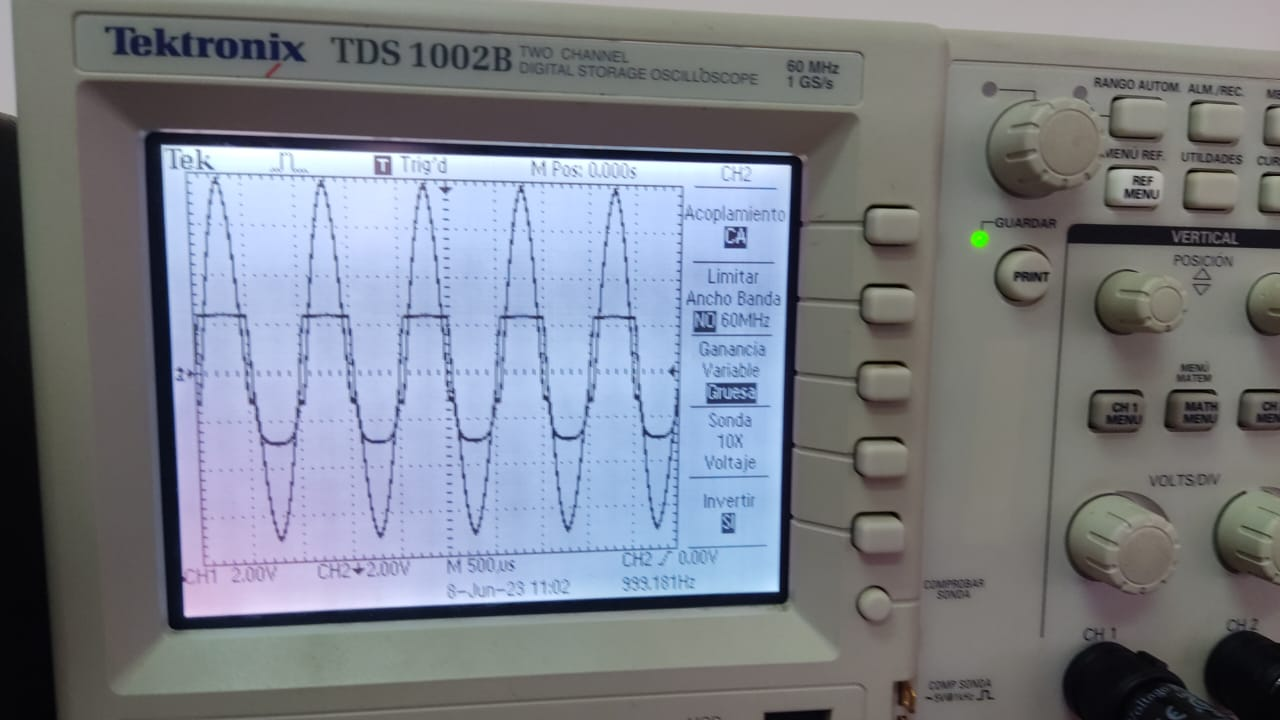
\includegraphics[width=12cm,height=7cm]{Img/lab_5_img_6}
		
		\item Voltaje en resistencia y diodo, modo xy, osciloscopio digital:
		
		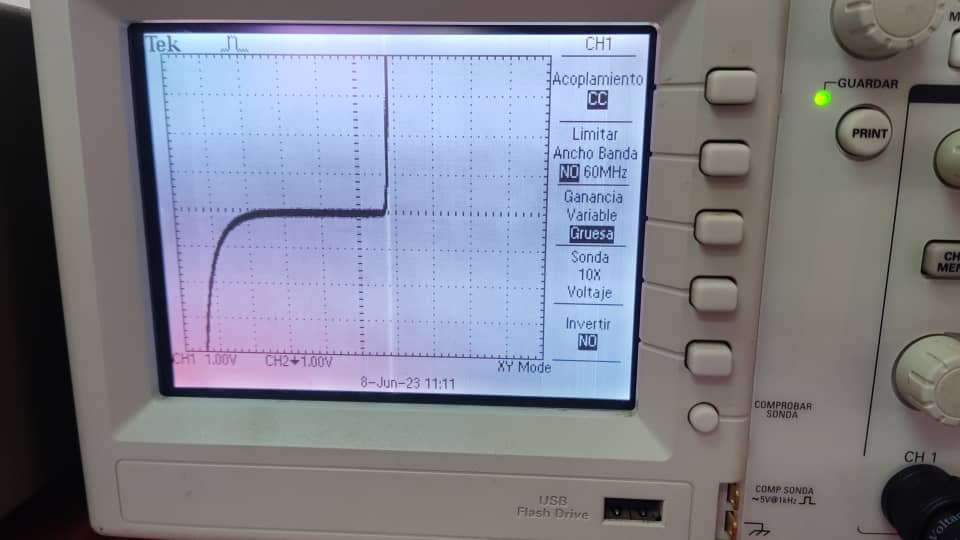
\includegraphics[width=12cm,height=7cm]{Img/lab_5_img_7}
		
		\item Voltaje en resistencia y diodo, modo xy, trazador de curvas:
		
		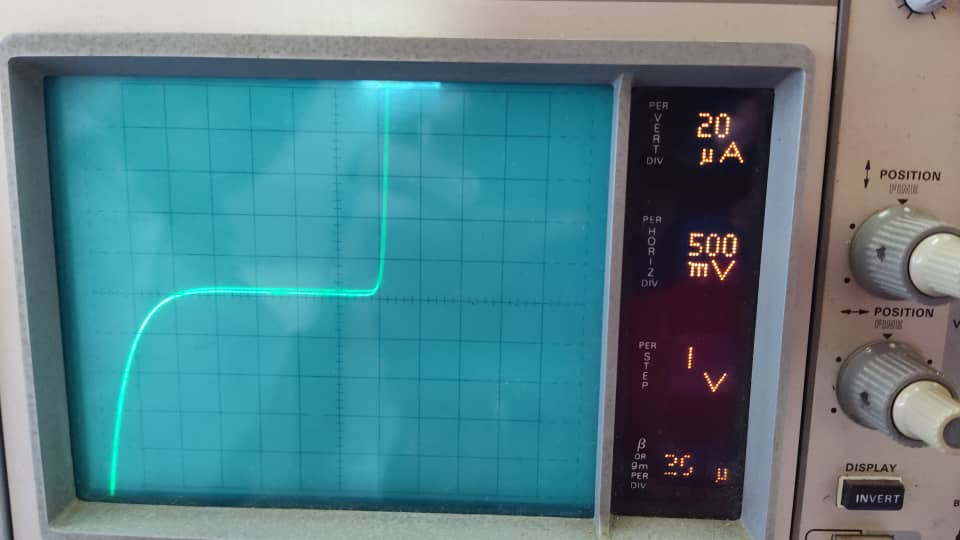
\includegraphics[width=12cm,height=7cm]{Img/lab_5_img_9}
		
		\item Voltaje en resistencia y diodo, modo xy, osciloscopio analógico:
		
		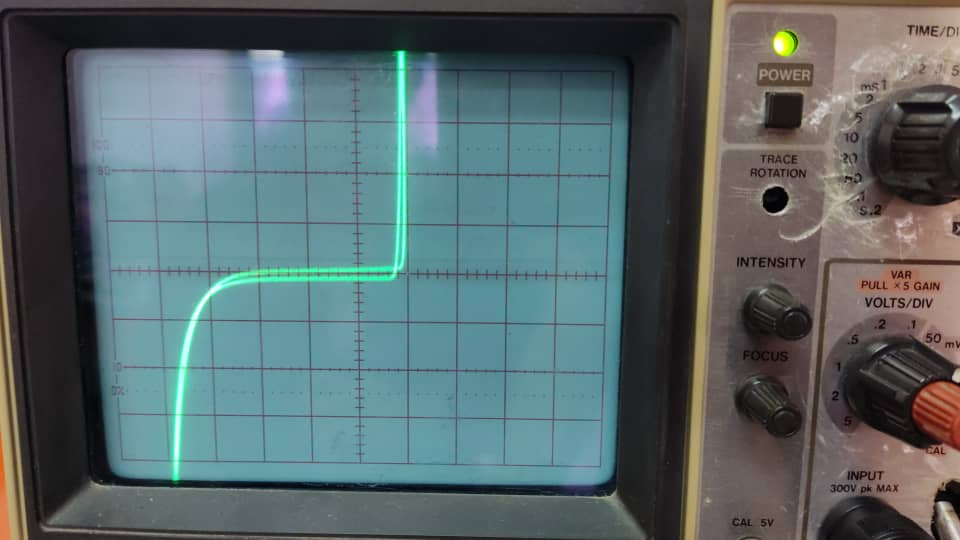
\includegraphics[width=12cm,height=7cm]{Img/lab_5_img_10}
		
	\end{enumerate}	
	
	\begin{center}
		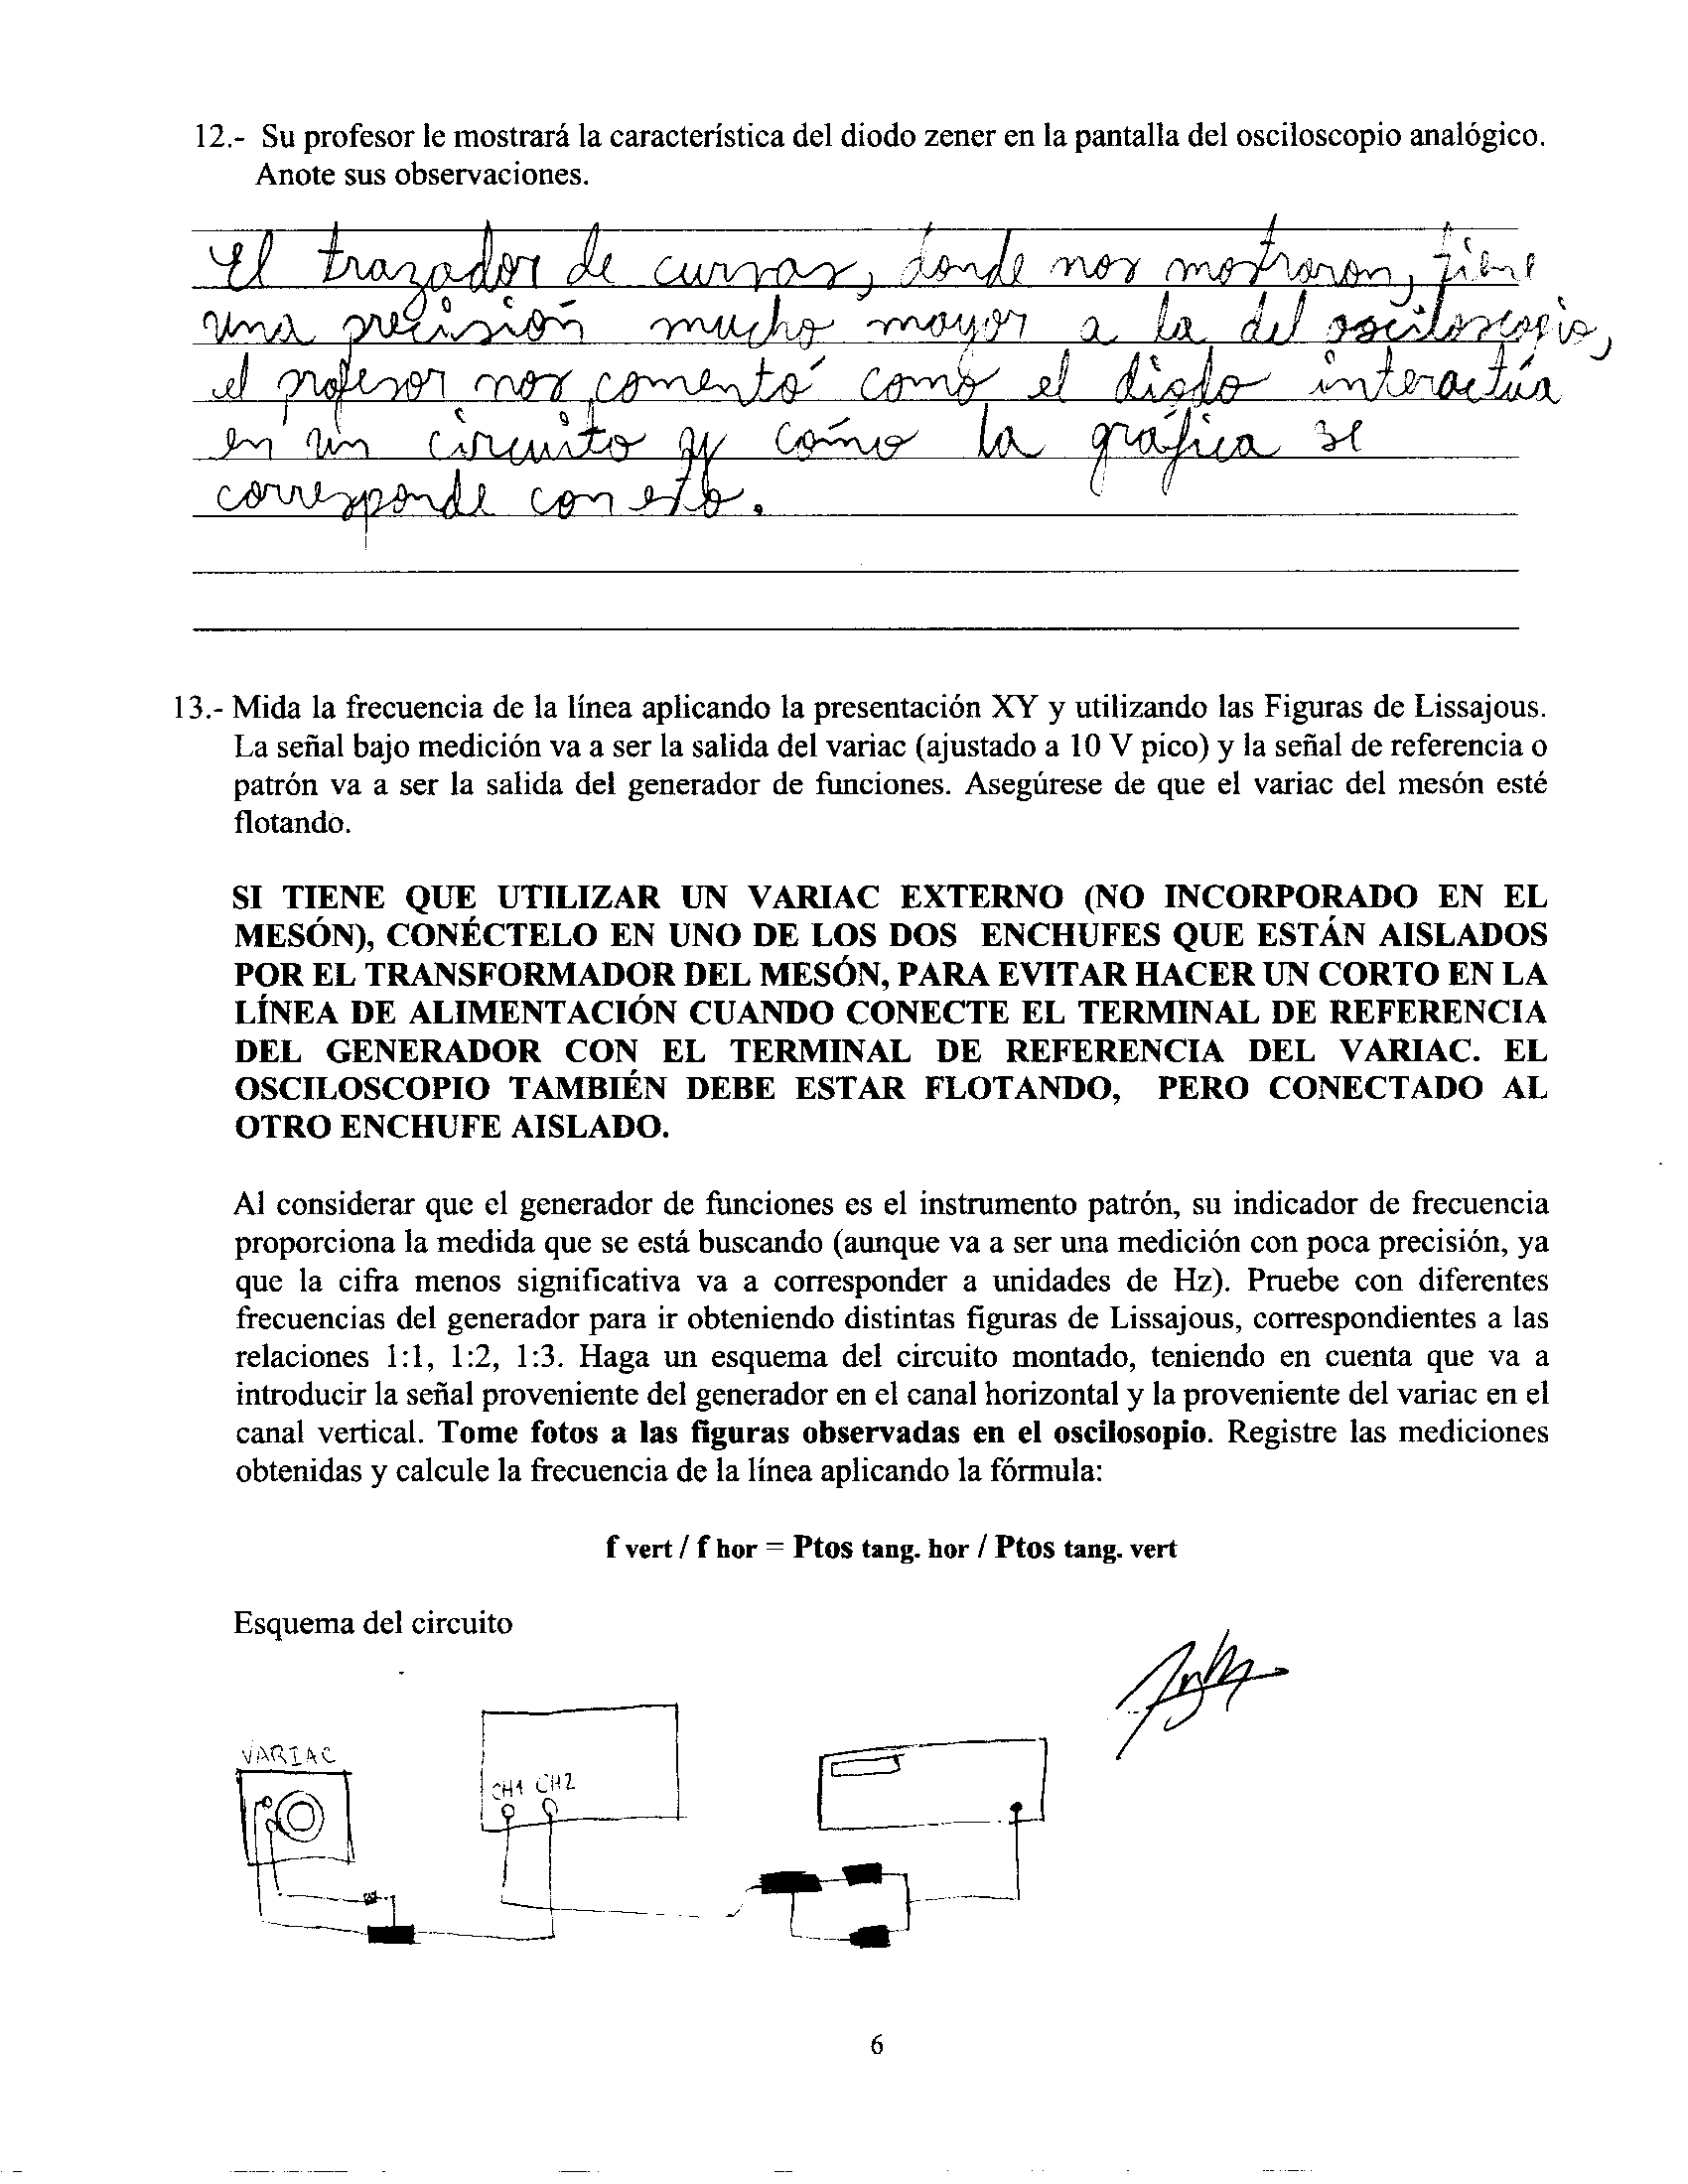
\includegraphics[width=16cm,height=20cm]{Img/anexo_0004}
	\end{center}
	
	\begin{center}
		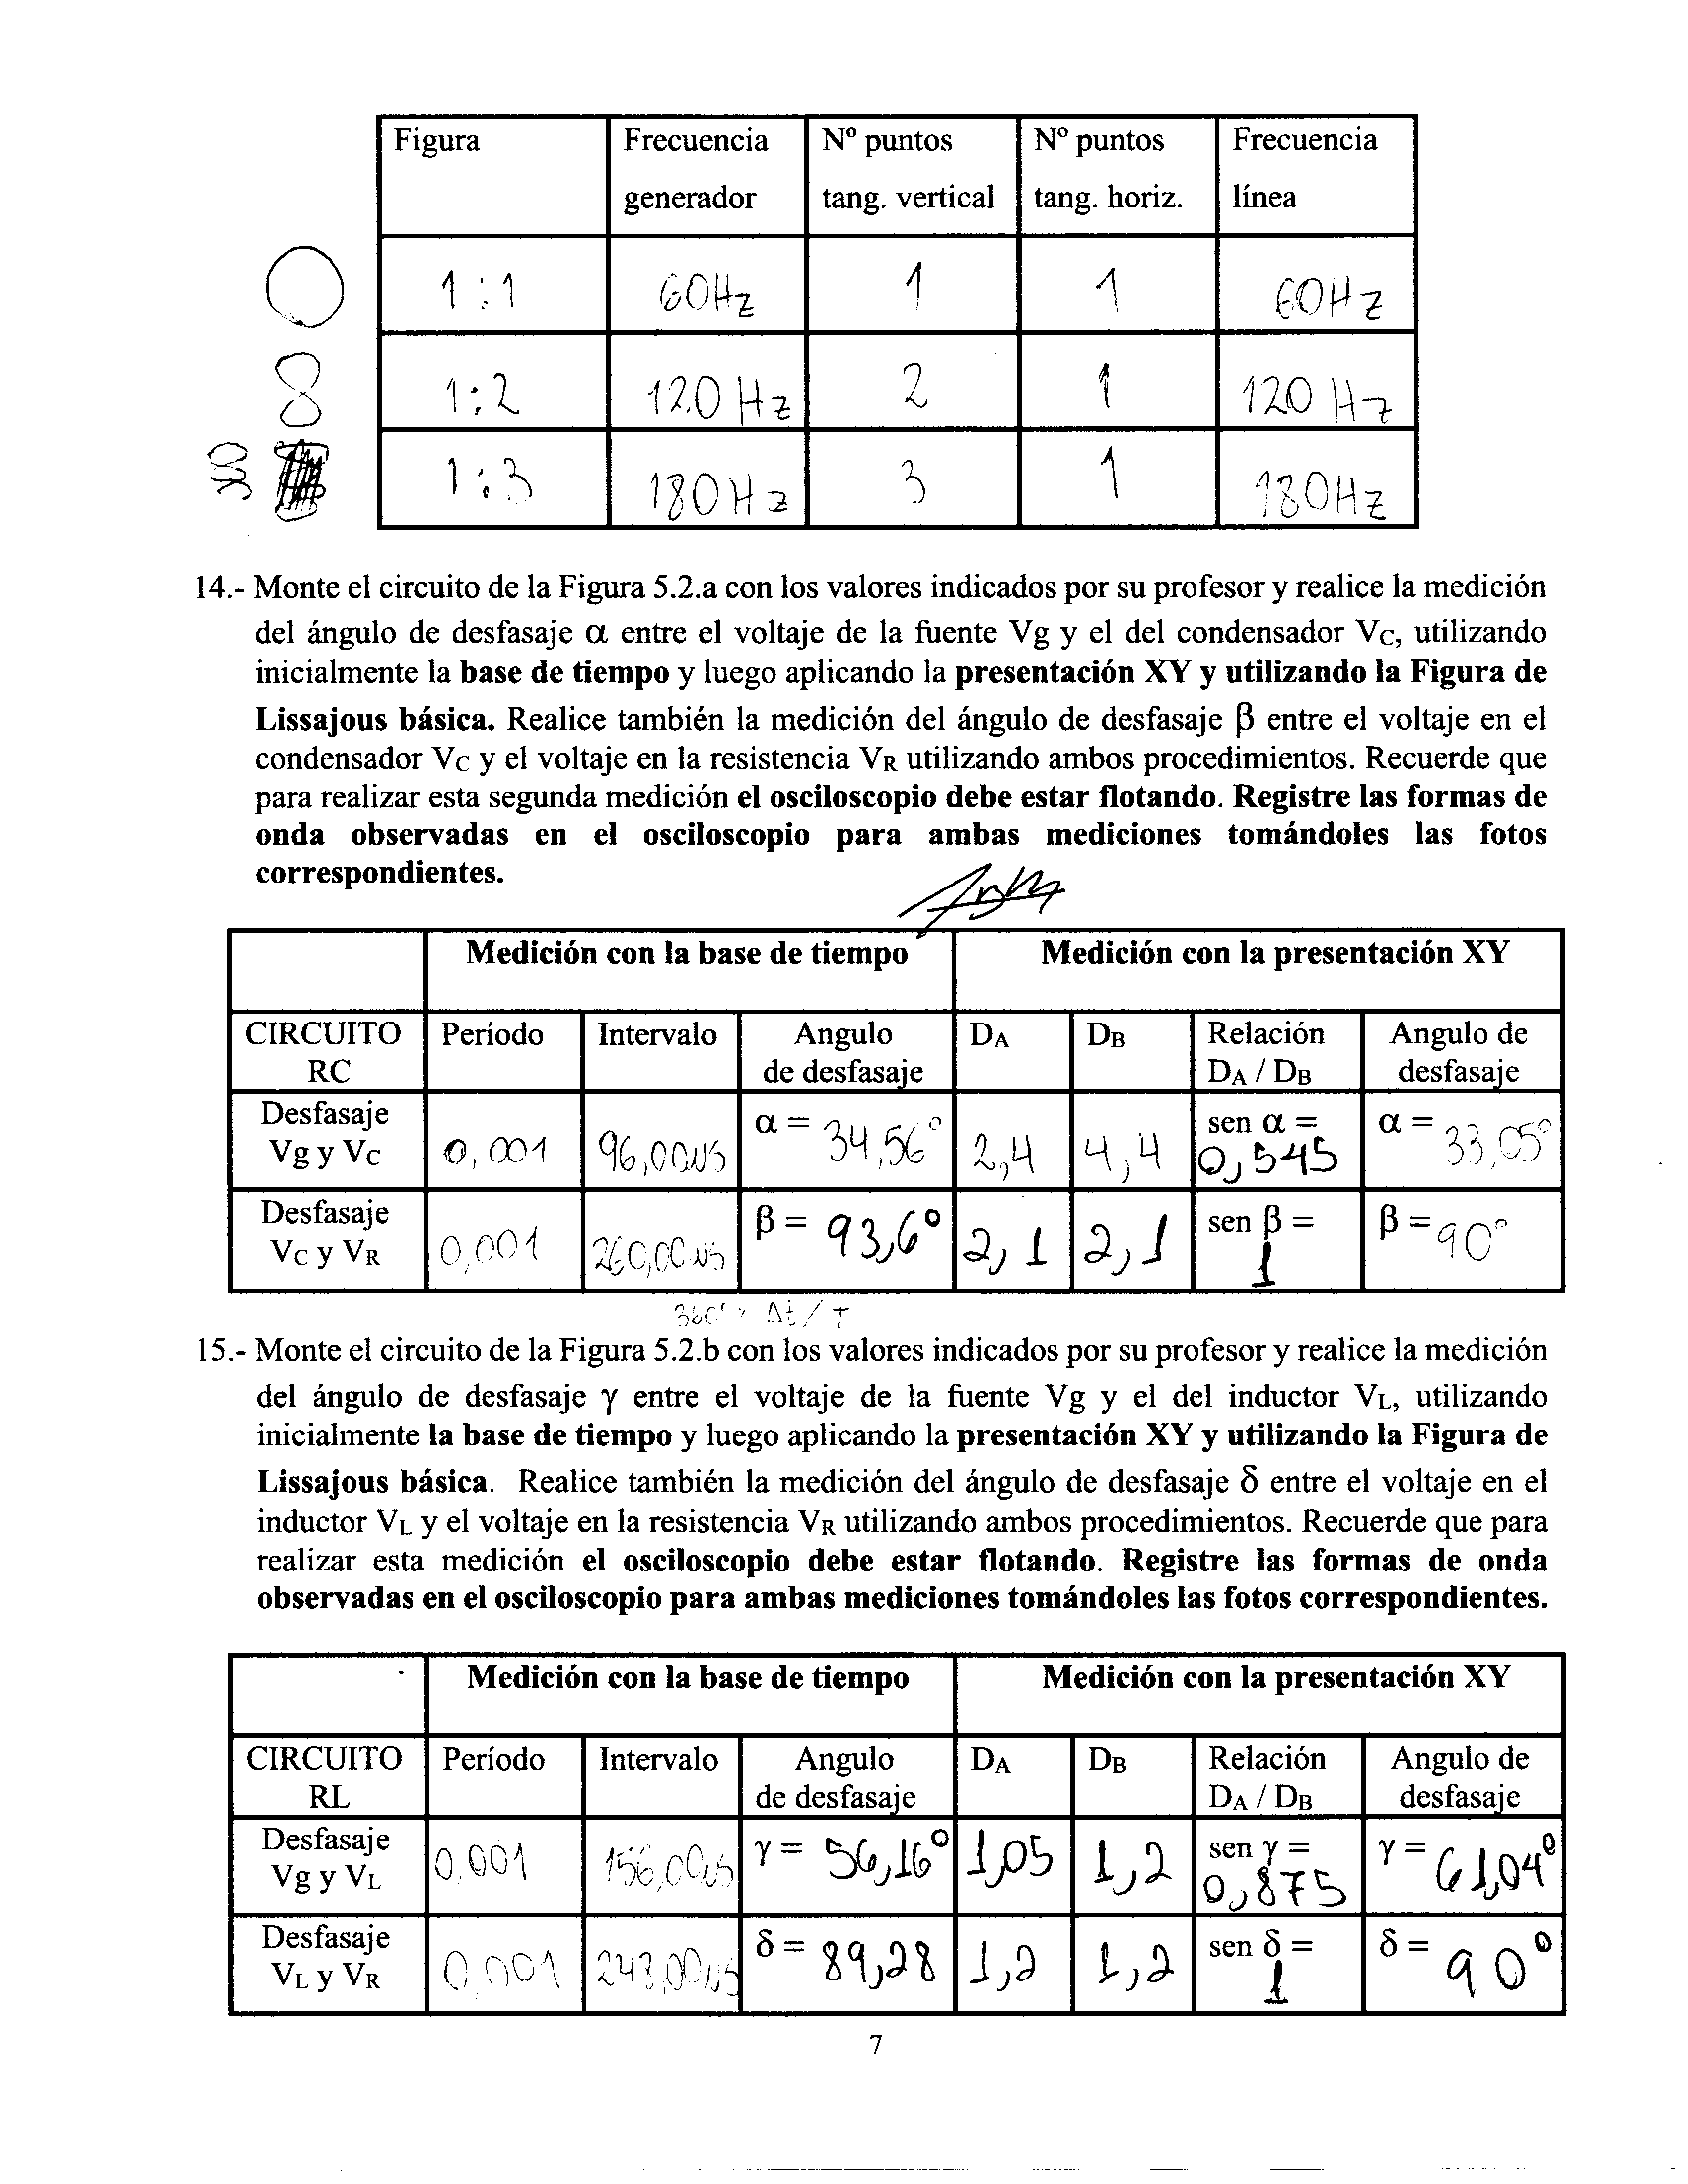
\includegraphics[width=16cm,height=20cm]{Img/anexo_0005}
	\end{center}
	
	\newpage
	
	\noindent Las imponentes figuras de Lissajous:
	
	\begin{enumerate}
		\item 1:1
		
		\begin{center}
			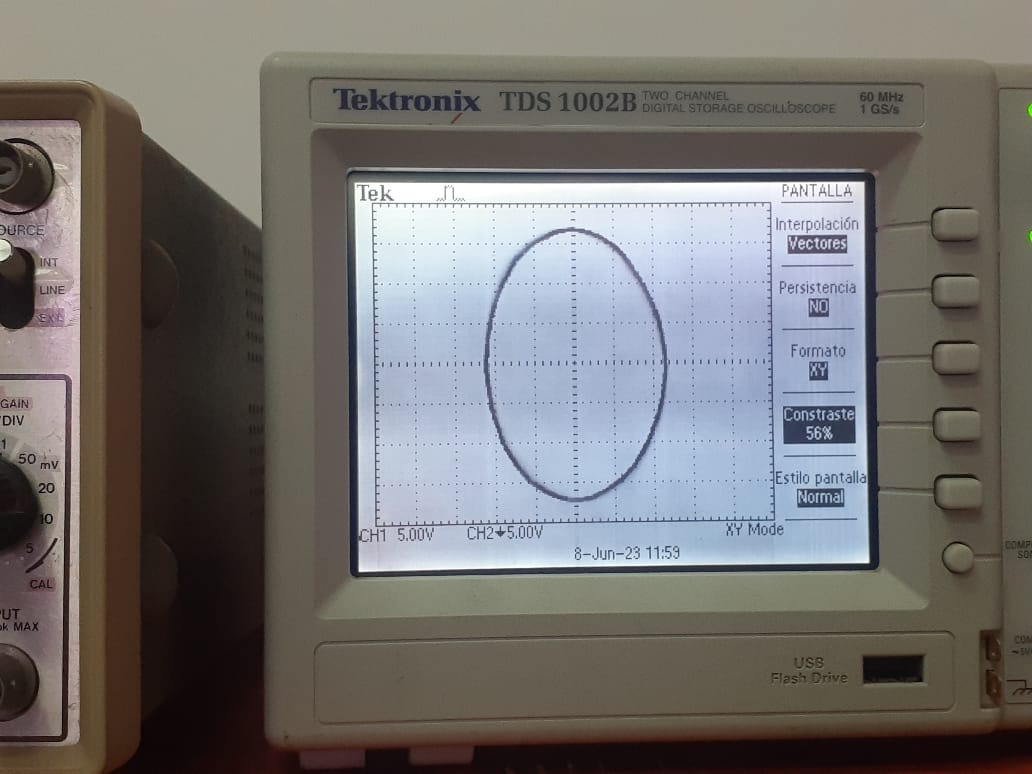
\includegraphics[width=12cm,height=8cm]{Img/l1}
		\end{center}
		
		\item 1:2
		
		\begin{center}
			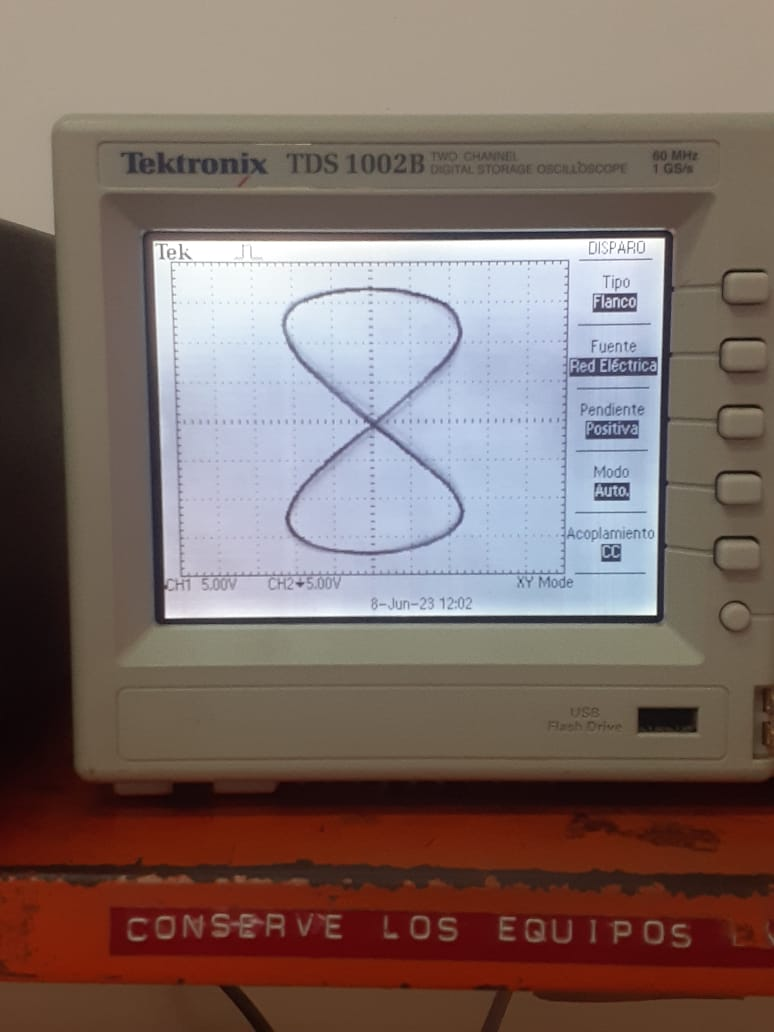
\includegraphics[width=12cm,height=12cm]{Img/l2}
		\end{center}
		
		\item 1:3
		
		\begin{center}
			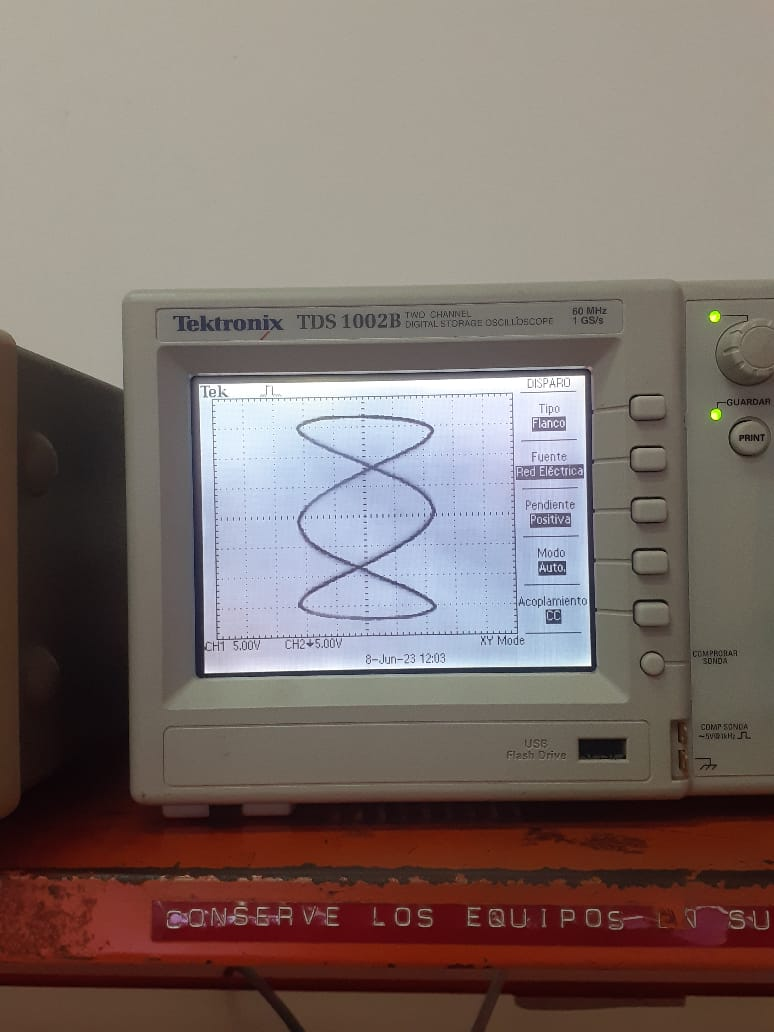
\includegraphics[width=12cm,height=12cm]{Img/l3}
		\end{center}
		
	\end{enumerate}
	
	\begin{center}
		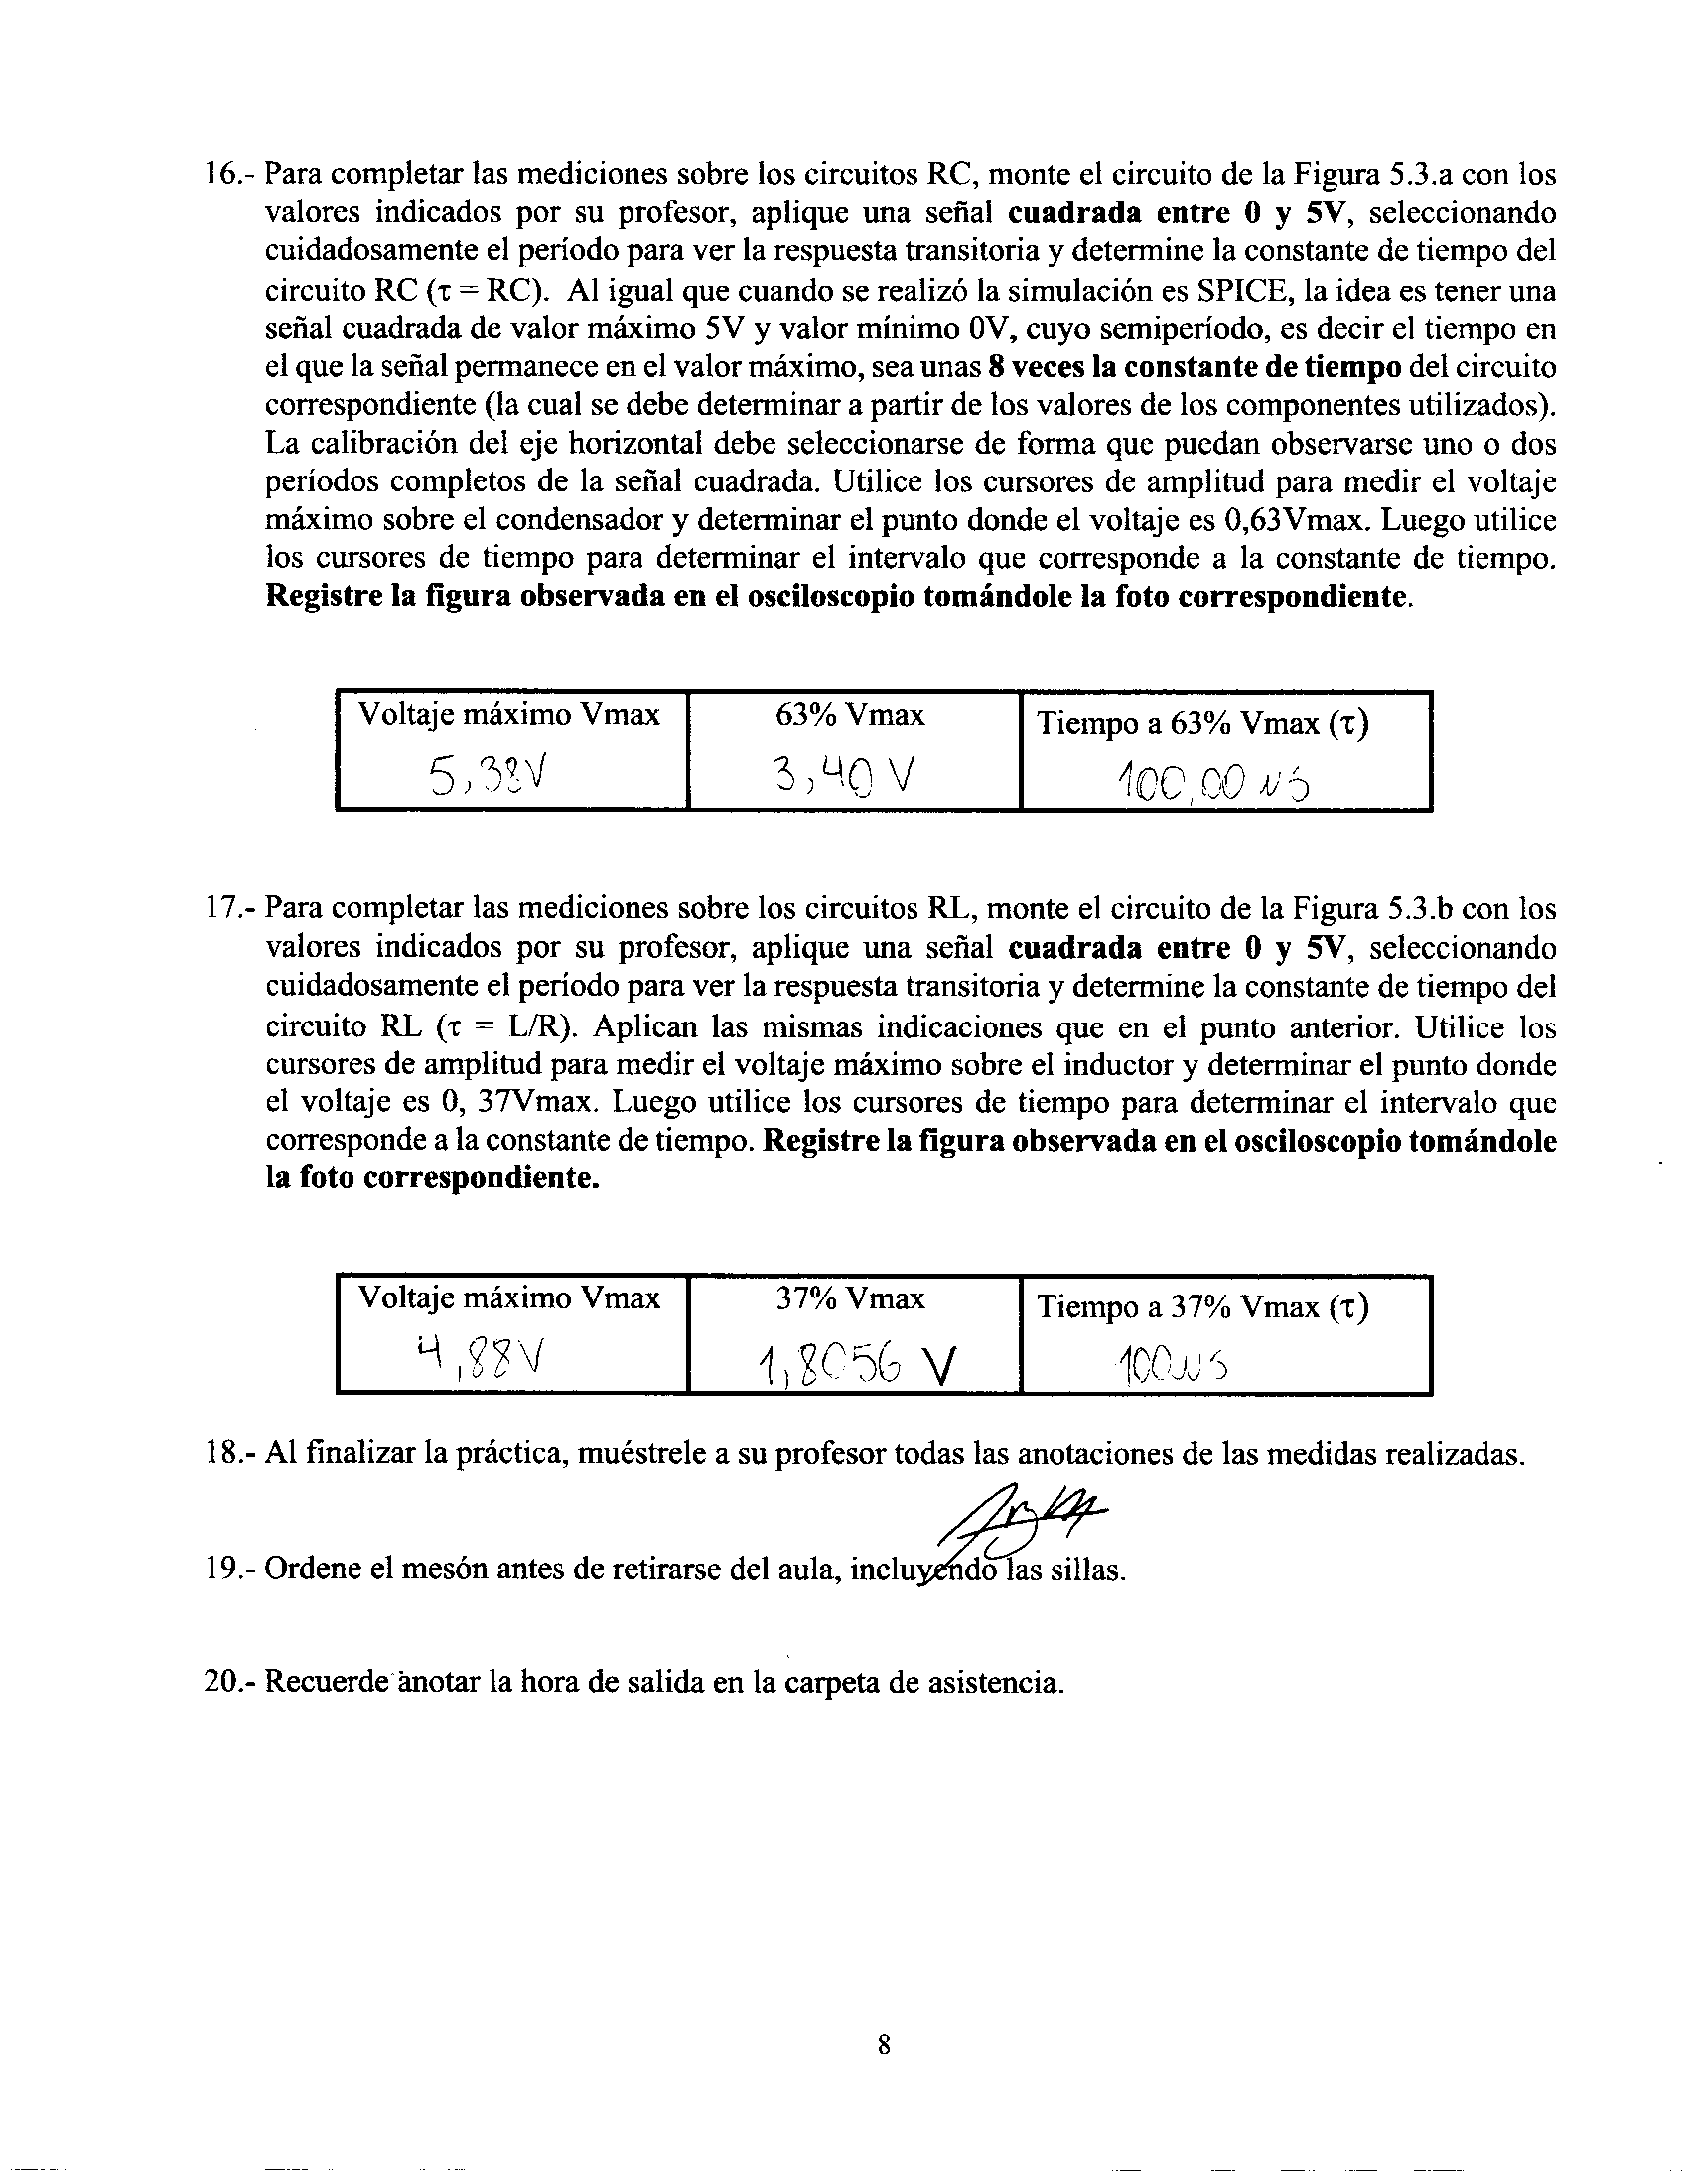
\includegraphics[width=16cm,height=20cm]{Img/anexo_0006}
	\end{center}
	
	\newpage
	
	\noindent Para las gráficas realizadas a partir de los valores medidos tendremos:
	
	
	\renewcommand{\theenumi}{\alph{enumi}} %Letras minúsculas 
	
	\begin{enumerate}
		\item Corriente vs voltaje en dos resistencias
		
		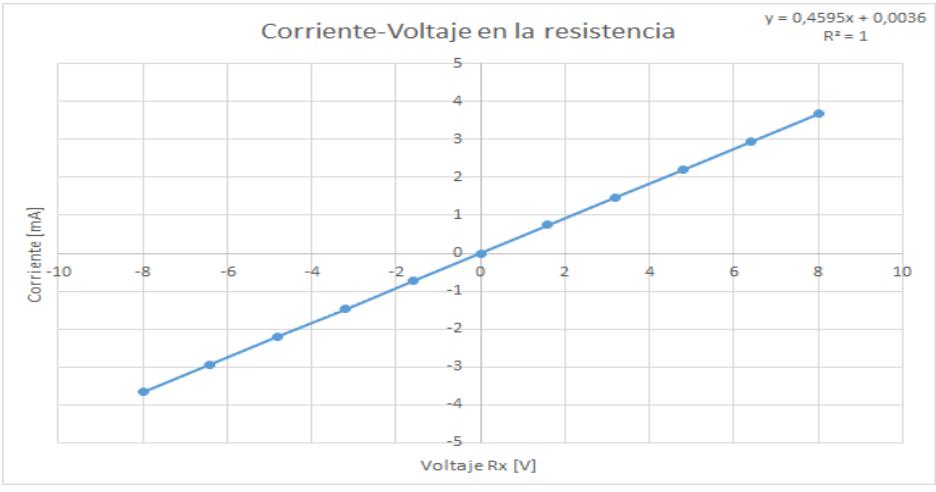
\includegraphics[width=12cm,height=8cm]{Img/graph_1}
		
		\noindent Se evidencia que hay una correlación entre el inverso multiplicativo de la pendiente y el valor de la resistencia, quedando:
		
		\begin{equation}
			\notag [m] = [\frac{mA}{V}] \Rightarrow [m^{-1}] = [\frac{V}{mA}] \Rightarrow R = \frac{1}{m} =  2,176k \Omega
		\end{equation}
		
		\noindent Quedando que el error respecto al valor nominal es:
		
		\begin{equation}
			\notag E\% = \frac{|2,176k\Omega - 2,2k\Omega|}{2,2k\Omega}\times 100\% = 1,09\% 
		\end{equation}
		
		\newpage
		
		\item Corriente vs voltaje en resistencia y diodo
		
		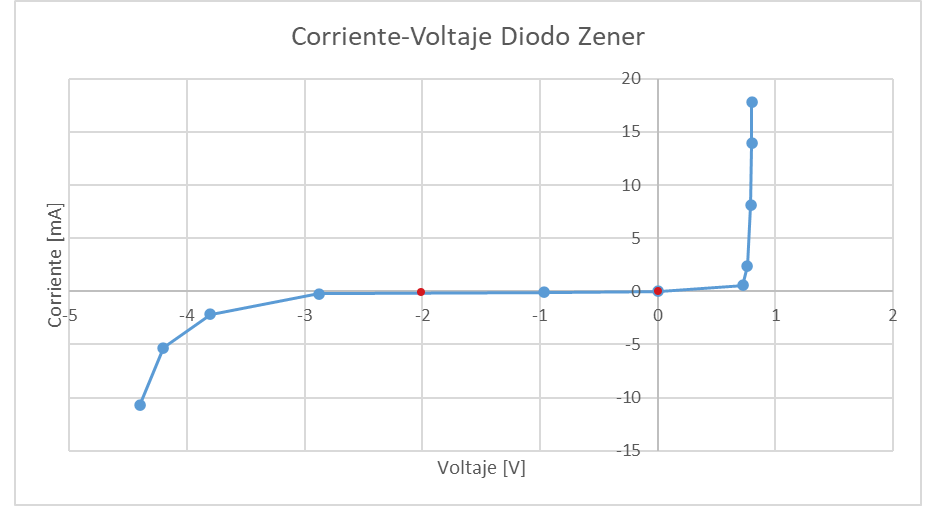
\includegraphics[width=12cm,height=8cm]{Img/graph_2}
		
		\noindent Los puntos rojos son donde aproximadamente empieza a conducir corriente el diodo, nótese que para polarización positiva del voltaje, se conduce corriente desde $0V$ mientra que para negativas hay un rango de valores en los ue la corriente circula muy poco o directamente no circula.
		
	\end{enumerate}
	
	\noindent Luego, al realizar lo cálculos tendremos:
	
	\renewcommand{\theenumi}{\alph{enumi}} %Letras minúsculas 
	
	\begin{enumerate}
		\item Error porcentual entre la frecuencia de línea medida y el valor nominal de $60Hz$:
		
		\begin{equation}
			\notag E\% = \frac{60Hz - 60Hz}{60Hz}\times 100\% = 0\%
		\end{equation}
		
		\item Circuito RC
		
		\noindent \textbf{Fuente y capacitor}
		
		\begin{center}
			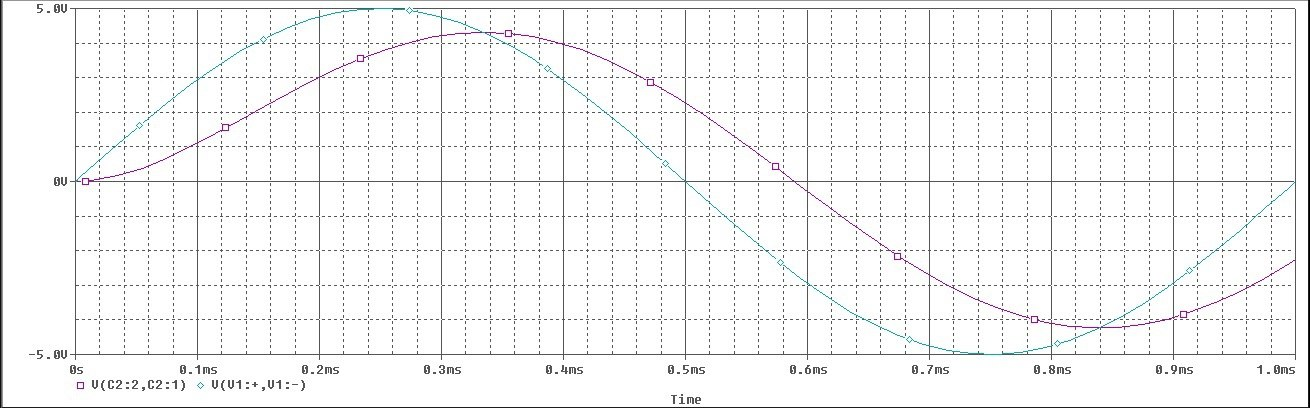
\includegraphics[width=16cm,height=8cm]{Img/spice_c_source}
		\end{center}
		
		\noindent Acá tenemos que $\Delta t = 0,59s - 0,5s = 0,09s\Rightarrow X^\circ = \frac{360 \times 0,09ms}{1ms} = 32,4^\circ$, así el error será:\\
		
		\noindent Para medición en el tiempo
		
		\begin{equation}
			\notag E\% = \frac{34,56^\circ - 32,4^\circ}{32,4^\circ}\times 100\% = 6,66\%
		\end{equation}
		
		\noindent Para medición XY
		
		\begin{equation}
			\notag E\% = \frac{33,05^\circ - 32,4^\circ}{32,4^\circ}\times 100\% = 2,01\%
		\end{equation}
		
		\noindent \textbf{Capacitor y resistencia}
		
		\begin{center}
			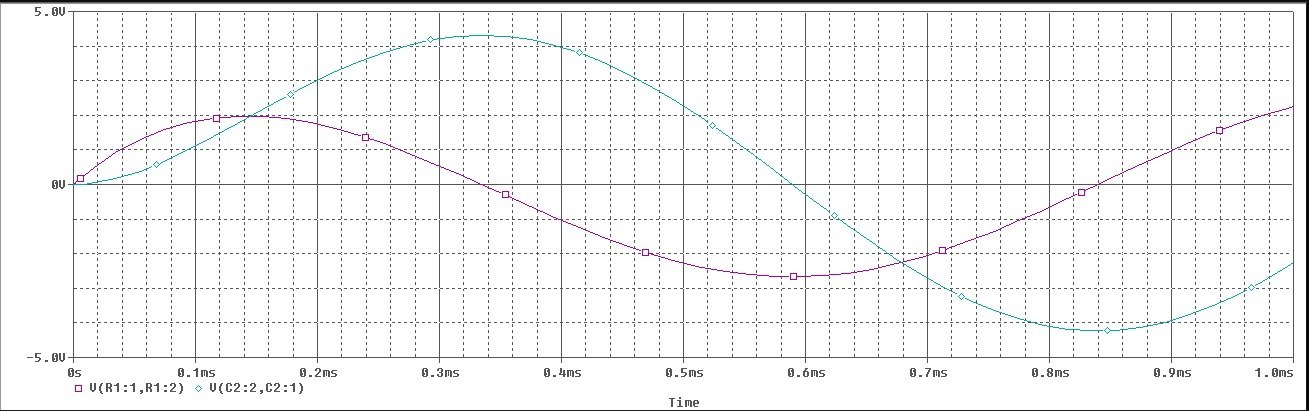
\includegraphics[width=16cm,height=8cm]{Img/spice_cvresist}
		\end{center}
		
		\noindent Se vislumbra que $\Delta t = 0,59s - 0,34s = 0,25s\Rightarrow X^\circ = \frac{360 \times 0,25ms}{1ms} = 90^\circ$
		
		\noindent Para medición en el tiempo
		
		\begin{equation}
			\notag E\% = \frac{93,6^\circ - 90^\circ}{90^\circ}\times 100\% = 4\%
		\end{equation}
		
		\noindent Para medición XY
		
		\begin{equation}
			\notag E\% = \frac{90^\circ - 90^\circ}{90^\circ}\times 100\% = 0\%
		\end{equation}
		
		\item Circuito RL
		
		\noindent \textbf{Fuente e inductor}
		
		\begin{center}
			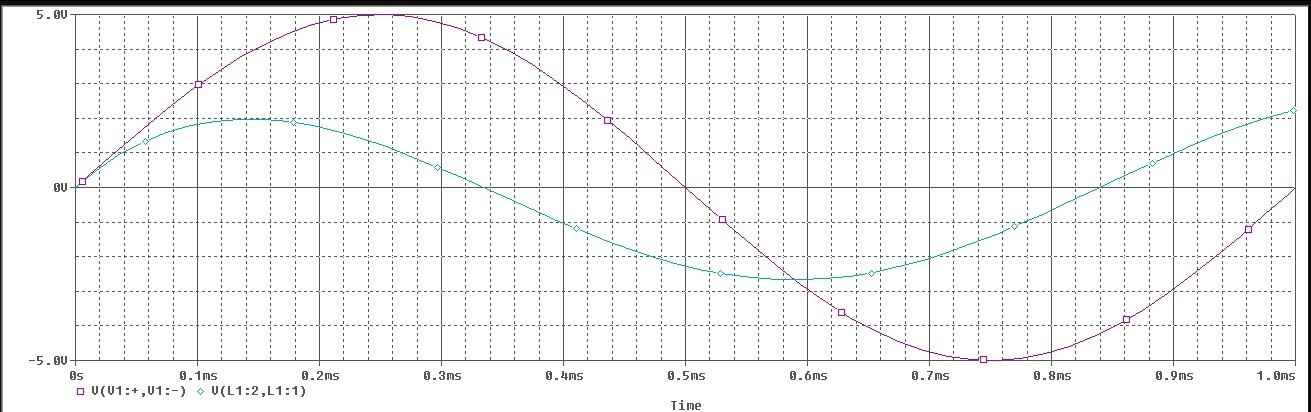
\includegraphics[width=16cm,height=8cm]{Img/spice_lvsource}
		\end{center}
		
		\noindent De allí se calcula $\Delta t = 0,5s - 0,34s = 0,16s\Rightarrow X^\circ = \frac{360 \times 0,16ms}{1ms} = 57,6^\circ$
		
		\noindent Para medición en el tiempo
		
		\begin{equation}
			\notag E\% = \frac{|56,16^\circ - 57,6^\circ|}{57,6^\circ}\times 100\% = 2,5\%
		\end{equation}
		
		\noindent Para medición XY
		
		\begin{equation}
			\notag E\% = \frac{61,04^\circ - 57,6^\circ}{57,6^\circ}\times 100\% = 5,97\%
		\end{equation}
		
		\noindent \textbf{Inductor y resistencia}
		
		\begin{center}
			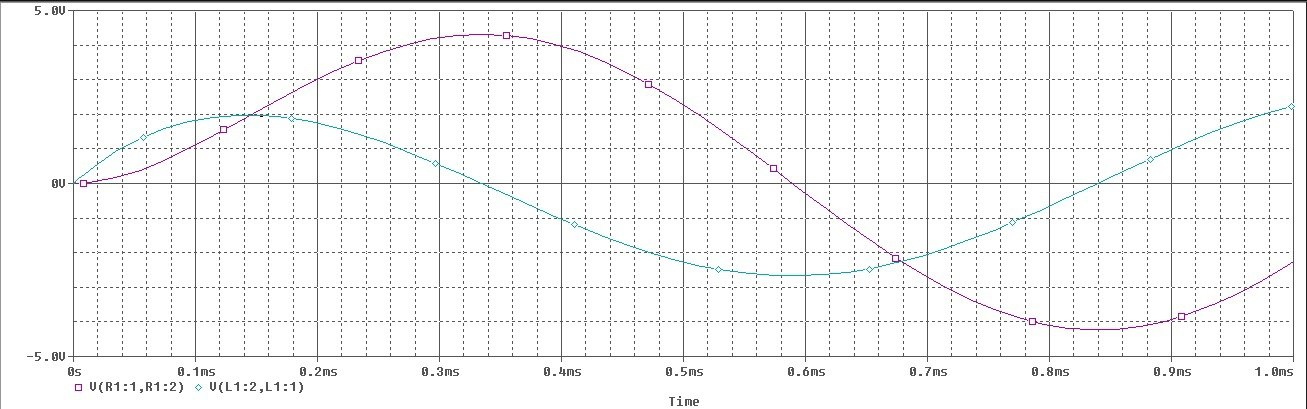
\includegraphics[width=16cm,height=8cm]{Img/spice_lvresist}
		\end{center}
		
		\noindent Entonces se obtiene $\Delta t = 0,59s - 0,34s = 0,25s\Rightarrow X^\circ = \frac{360 \times 0,25ms}{1ms} = 90^\circ$
		
		\noindent Para medición en el tiempo
		
		\begin{equation}
			\notag E\% = \frac{|89,28^\circ - 90^\circ|}{90^\circ}\times 100\% = 0,8\%
		\end{equation}
		
		\noindent Para medición XY
		
		\begin{equation}
			\notag E\% = \frac{90^\circ - 90^\circ}{90^\circ}\times 100\% = 0\%
		\end{equation}
		
		\item Constantes de tiempo
		
		\noindent \textbf{Capacitor}
		
		\begin{center}
			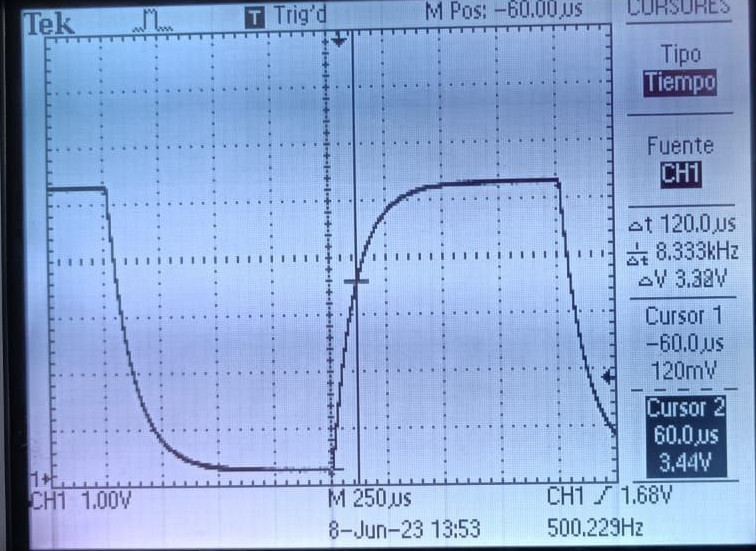
\includegraphics[width=16cm,height=8cm]{Img/capacitor}
		\end{center}
		
		\noindent De allí se evidencia que la constante de tiempo $\tau$ es de $120\mu s$ para nuestra medición, mientras que para la simulación
		
		\begin{center}
			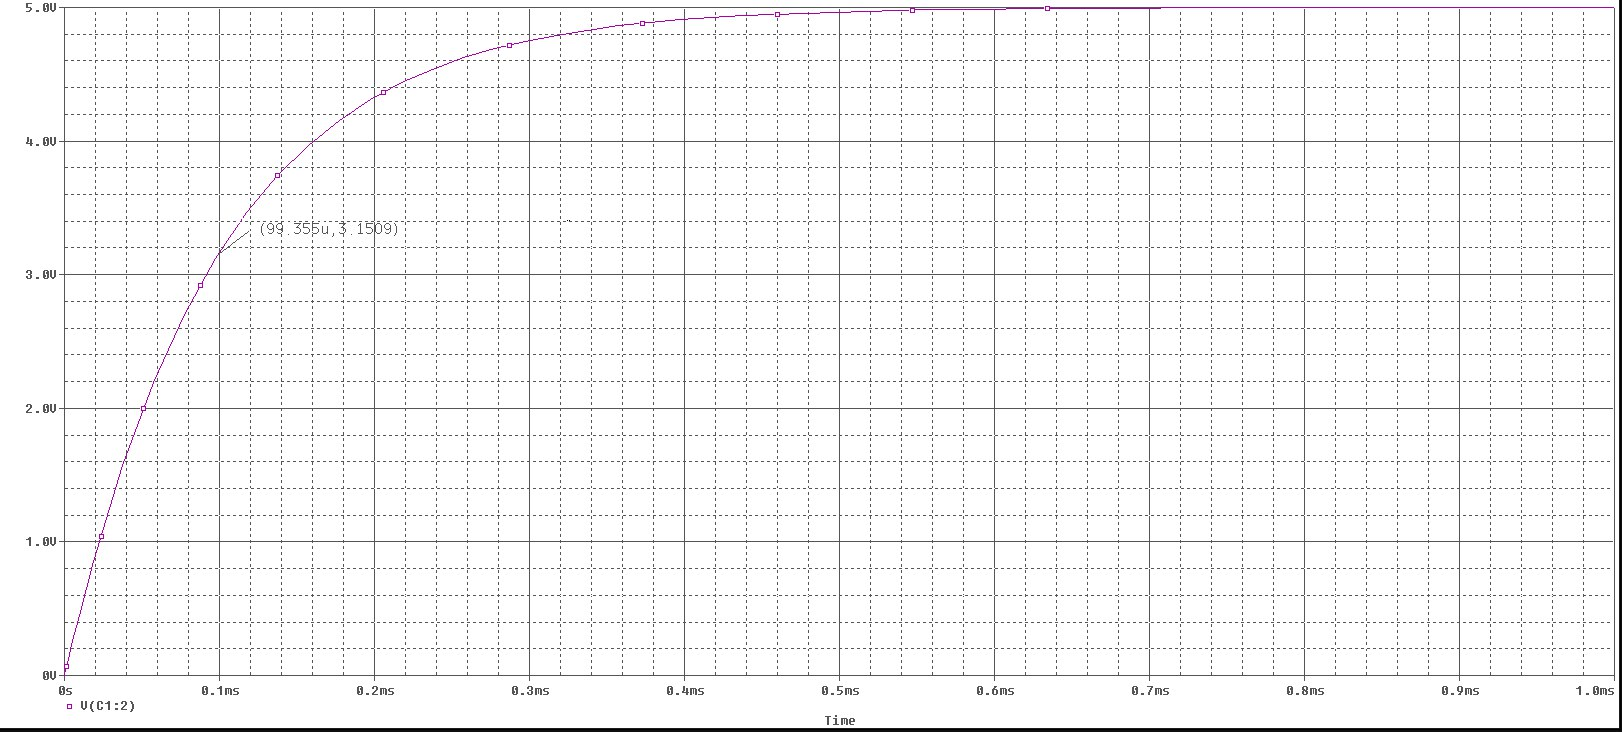
\includegraphics[width=16cm,height=8cm]{Img/capacitor_spice}
		\end{center}
		
		\noindent Se evidencia que en spice $\tau = 99,355 \mu s$
		
		\begin{equation}
			\notag E\% = \frac{120 - 99,355}{99,355}\times 100\% = 20,77\%
		\end{equation}
		
		\noindent Lo cual representa un error alto.
		
		\noindent \textbf{Inductor}
		
		\begin{center}
			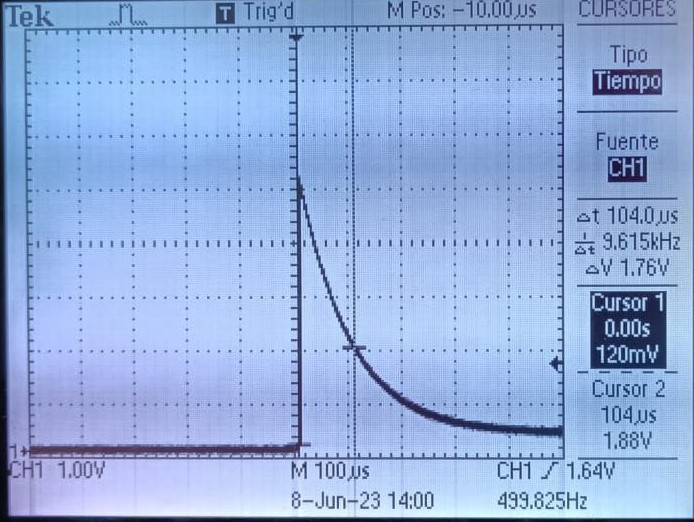
\includegraphics[width=16cm,height=8cm]{Img/inductor}
		\end{center}
		
		\noindent Obtenemos $\tau = 104 \mu s$ en el osciloscopio, mientras que para la simulación:
		
		\begin{center}
			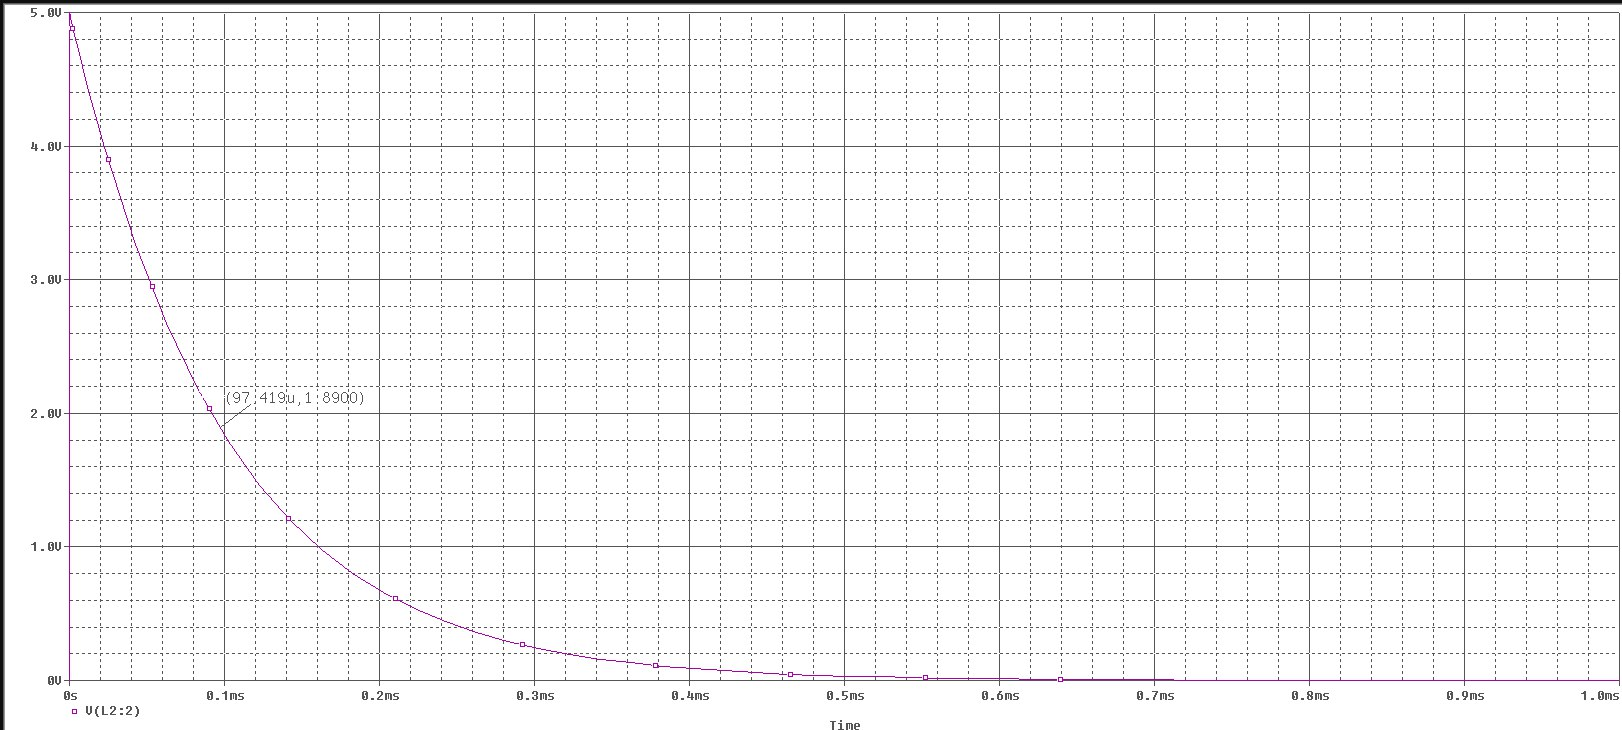
\includegraphics[width=16cm,height=8cm]{Img/inductor_spice}
		\end{center}
		
		\noindent Luego, queda claro que $\tau = 97,914 \mu s$ para la simulación de spice
		
		\begin{equation}
			\notag E\% = \frac{104 - 97,914}{97,914}\times 100\% = 6,22\%
		\end{equation}
		
		\noindent Un error bastante más bajo que el anterior.
		
	\end{enumerate}
	
	\newpage
	
	\begin{center}
		\textbf{\large ANÁLISIS DE RESULTADOS}\\
	\end{center}
	
	\renewcommand{\theenumi}{\alph{enumi}} %Letras minúsculas 
	
	\begin{enumerate}
		\item Gráficas de $R_x$:
		
		\noindent La pendiente de la recta de $R_x$ calculada en excel es bastante aproximada a la obtenida en el osciloscopio ya que esta resultó ser $0,4595$ mientras que la del osciloscopio fue $0,4545$, cabe a destacar que la del osciloscopio se calculó observando la gráfica, por lo que puede haber errores debido a una observación no perfecta.
		
		\item Diodo zener:
		
		\noindent En el caso del diodo zener, se pudo estudiar desde los dos osciloscopios y el trazador de curvas, todas las gráficas fueron la misma, sin embargo la más exacta y precisa fue la del trazador de curvas, la gráfica creada en excel también es una excelente representación de las medidas del diodo zener. Claramente se vió que el diodo zener estudiado era de $4,3V$ y se observó claramente como para valores de voltaje negativos muy bajos el diodo no conduce corriente, mientras que para voltajes positivos la conduce exponencialmente desde bajos voltajes.
		
		\item Gráficas RC y RL:
		
		\noindent Para el caso de estas gráficas se evidencia una gran similitud con respecto a la simulaciones, como siempre, en la práctica las señales pueden tener ruido y se tienen distintos efectos que quizá hagan que las señales tengan diferencias mínimas respecto a sus contrapartes en spice. Respecto a los errores, fueron bastante bajo, en el caso de los inductores el error era por defecto y en los capacitores por exceso. Las fotos del osciloscopio para este inciso estarán en los anexos.
	\end{enumerate}
	
	\newpage
	
	\begin{center}
		\textbf{\large CONCLUSIONES}\\
	\end{center}
	
	\noindent Esta práctica tuvo como objetivo aprender a utilizar el modo XY de los osciloscopios para realizar mediciones en distintos componentes, además, se estudió la precisión y exactitud del mismo. El modo XY es sumamente útil para vislumbrar el comportamiento de un elemento tomando la variación de corriente en función del cambio de voltaje, permite estudiar y caracterizar una extensa gama de componentes.\\
	
	\noindent También se estudiaron los circuitos RL y RC vistos anteriormente en la práctica de spice, para luego comparar cómo fluctuan los valores ideales de spice respecto a la medición de un circuito real. Se evidenció que los resultados son sumamente precisos y exactos, con pequeñas fluctuaciones que no superaron el $7\%$ de error. Sin duda se confirma que el osciloscopio es una herramienta indispensable al estudiar señales.\\
	
	\noindent En el caso de las constantes de tiempo se pudo evidenciar que en el caso del inductor el error fue mucho menor que en el capacitor, se sospecha que esto se debe a que al tomar la foto del capacitor no se ubicó correctamente los cursores.\\
	
	\noindent La primera aproximación al diodo zener en toda la carrera se dió en esta práctica, pudiendo apreciar cómo interactúan los elementos no lineales de un circuito con la corriente y el voltaje, es un cambio respecto a lo que se había estudiado hasta ahora en la parte eléctrica, donde habíamos estudiado elementos lineales como las resistencias.\\
	
	\noindent No cabe duda de que desarrollar las prácticas de laboratorio desarrolla cierta madurez en los estudiantes y permite que se conozca cómo se desenvuelven los fenómenos que ya se han estudiado en un circuito funcionando, es indispensable el manejo de estos conocimientos prácticos para aclarar ideas y cimentar otras presentes durante el estudio de la electricidad.
	
	
	\newpage
	
	\begin{center}
		\textbf{\large BIBLIOGRAFÍA}\\
	\end{center}
	
	\noindent Guía Teórica versión electrónica, ubicada en la página web del laboratorio C, http://www.labc.usb.ve,
	enlace a "Página web de Asignaturas”, EC1282- Laboratorio de Circuitos 2013.
	
	\newpage
	
	\begin{center}
		\textbf{\large ANEXOS}\\
	\end{center}
	
	\textit{Figura 1. Ondas sinosoidales: Capacitor-Fuente}
	\begin{center}
		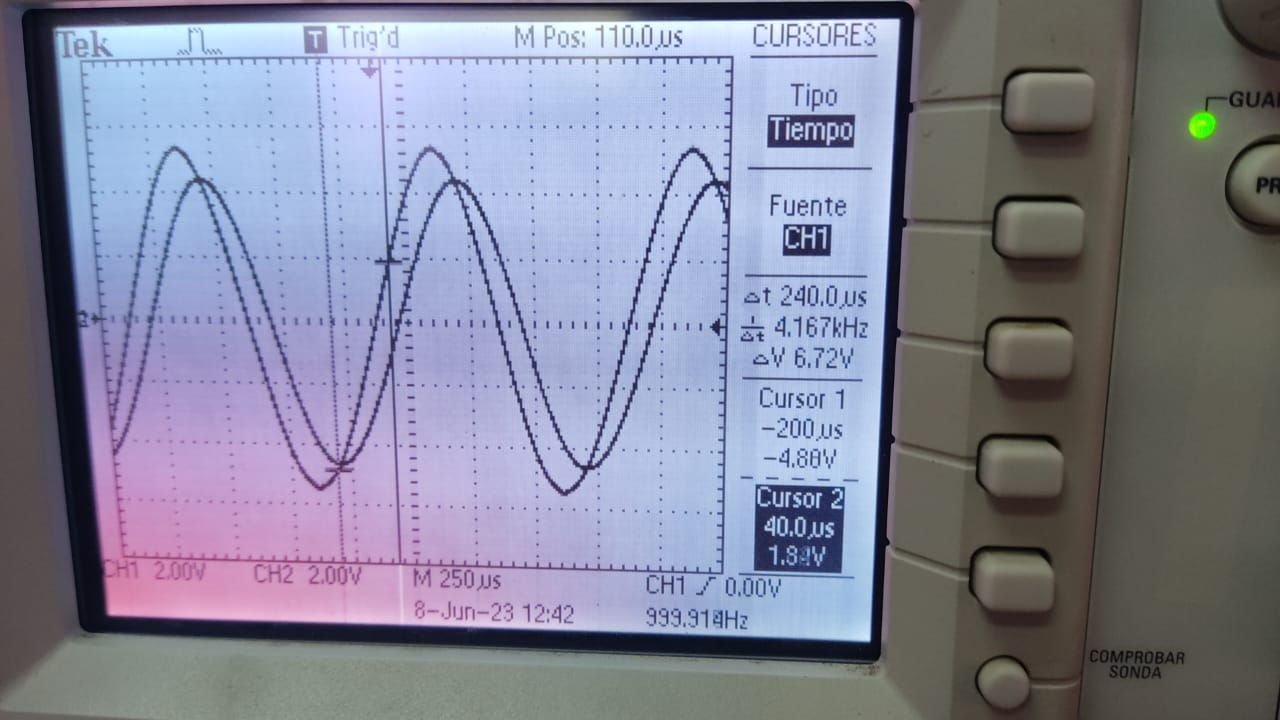
\includegraphics[width=12cm,height=7cm]{Img/lab_5_img_12}
	\end{center}
	
	\vspace{2cm}
	
	\textit{Figura 2. Ondas sinosoidales: Capacitor-Resistencia}
	\begin{center}
		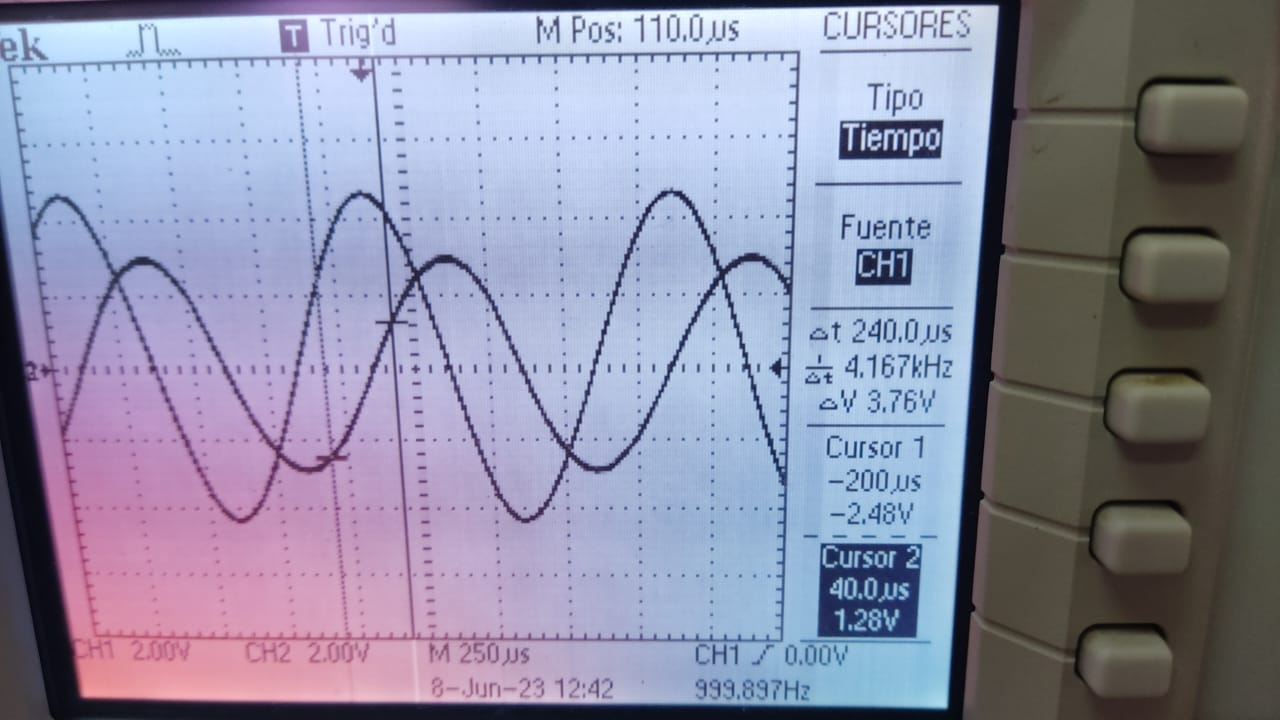
\includegraphics[width=12cm,height=7cm]{Img/lab_5_img_13}
	\end{center}
	
	\newpage
	
	\textit{Figura 3. Ondas sinosoidales: Fuente-Inductor}
	\begin{center}
		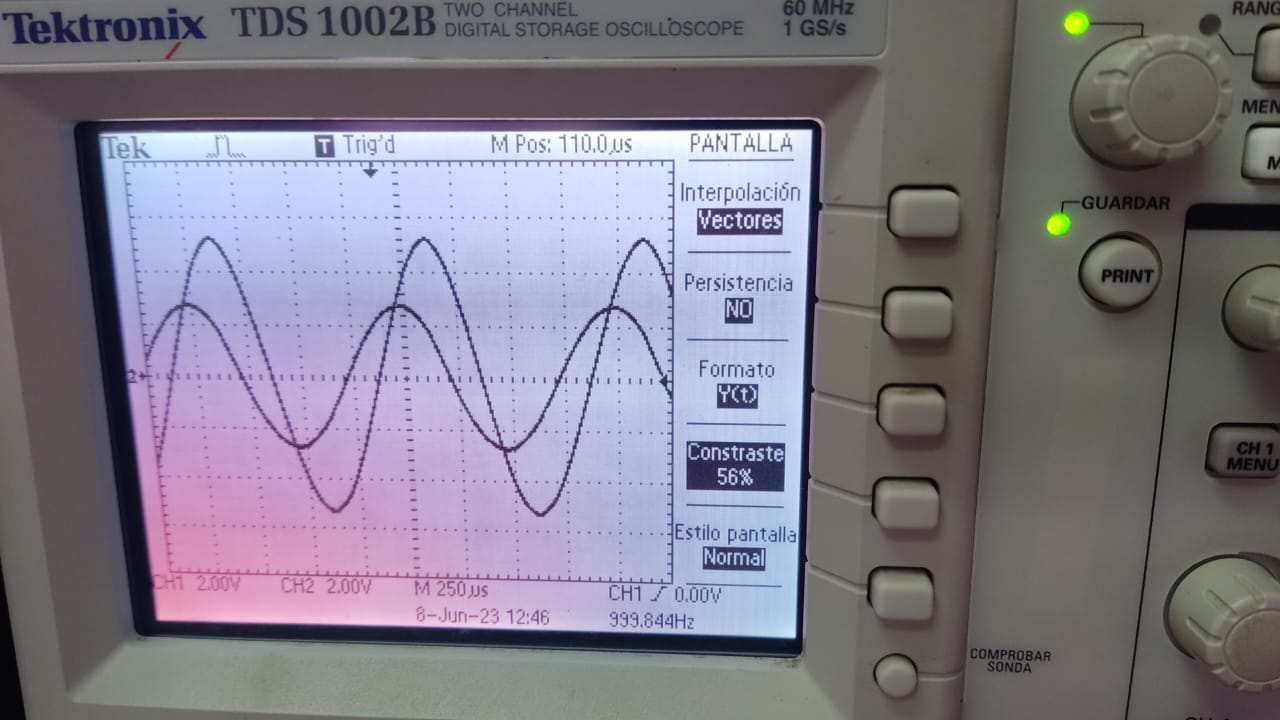
\includegraphics[width=12cm,height=7cm]{Img/lab_5_img_15}
	\end{center}
	
	\vspace{2cm}
	
	\textit{Figura 4. Ondas sinosoidales: Inductor-Resistencia}
	\begin{center}
		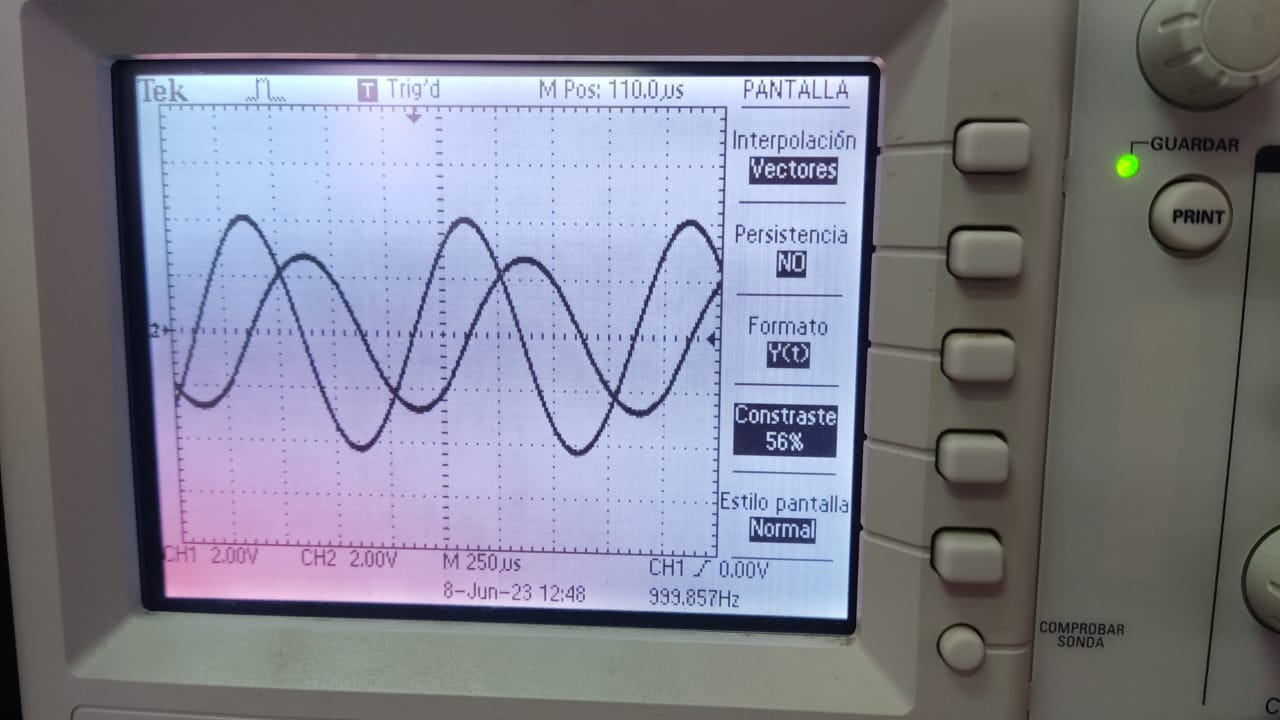
\includegraphics[width=12cm,height=7cm]{Img/lab_5_img_17}
	\end{center}
	
\end{document}